% \documentclass[conference]{IEEEtran}
%temp
\documentclass[a4paper]{article} 
\usepackage{cite}
\usepackage{amsmath,amssymb,amsfonts,amsthm}
\usepackage{algorithmic}
\usepackage{graphicx}
\usepackage{tabularx}
\usepackage{textcomp}
\usepackage[dvipsnames,table]{xcolor}
\usepackage{array}
\usepackage{mdframed}
\usepackage[most]{tcolorbox}
\usepackage{hyperref}
%temp package
\usepackage[colorinlistoftodos]{todonotes}
\usepackage[margin=1in]{geometry}
\usepackage{enumitem}



% Formatting for links
% \hypersetup{
%     colorlinks=true,
%     citecolor=Blue, 
%     linkcolor=Maroon,
%     urlcolor=NavyBlue
% }


\newtheoremstyle{boldstyle}% name
  {\topsep}% space above
  {\topsep}% space below
  {\itshape}% body font
  { }% indent
  {\bfseries}% head font (bold!)
  {.}% punctuation after head
  { }% space after head
  {\thmname{#1}\thmnumber{ #2}\thmnote{ (#3)}}% head spec
\theoremstyle{boldstyle}
% \newtheorem{openquestionx}{Open Question}[section]
% \renewcommand{\theopenquestionx}{\thesection.Q\arabic{openquestionx}}
\newtheorem{openquestionx}{Open Question}
\renewcommand{\theopenquestionx}{Q\arabic{openquestionx}}
\newmdenv[
  skipabove=2pt,
  skipbelow=2pt,
  linewidth=1pt,
  linecolor=blue,
  backgroundcolor=blue!5,
  roundcorner=5pt,
  innertopmargin=2pt,
  innerbottommargin=2pt,
  innerleftmargin=3pt,
  innerrightmargin=3pt
]{openboxq}
\newenvironment{openquestion}
  {\begin{openboxq}\begin{openquestionx}}
  {\end{openquestionx}\end{openboxq}}

% Definition box formatting
\newtheorem{definitionx}{Definition} 
\newmdenv[
  skipabove=2pt,
  skipbelow=2pt,
  linewidth=1pt,
  linecolor=orange,
  backgroundcolor=orange!5,
  roundcorner=5pt,
  innertopmargin=2pt,
  innerbottommargin=2pt,
  innerleftmargin=3pt,
  innerrightmargin=3pt
]{defopenboxq}

\newenvironment{definition}
  {\begin{defopenboxq}\begin{definitionx}}
  {\end{definitionx}\end{defopenboxq}}
%%%%%%% 

\def\BibTeX{{\rm B\kern-.05em{\sc i\kern-.025em b}\kern-.08em
    T\kern-.1667em\lower.7ex\hbox{E}\kern-.125emX}}

% Caveat box formatting 
\newlength{\entrysep}
\setlength{\entrysep}{8pt}
%\par\vspace{\entrysep}

\newtcolorbox{riskbox}[1]{
                colback=black!6,
                colframe=black!35,
                colbacktitle=red!20,
                coltitle=black,
                fonttitle=\bfseries,
                title=#1,
                sharp corners,
                boxrule=0.2mm,
                boxsep=5pt,
                top=2pt,
                bottom=2pt,
                left=2pt,
                right=2pt
            }

\newtcolorbox{considerationbox}[1]{
                colback=black!6,
                colframe=black!35,
                colbacktitle=blue!20,
                coltitle=black,
                fonttitle=\bfseries,
                title=#1,
                sharp corners,
                boxrule=0.2mm,
                boxsep=5pt,
                top=2pt,
                bottom=2pt,
                left=2pt,
                right=2pt
            }

% \newtcolorbox{caveatbox}[1]{
%                 colback=black!5,
%                 colframe=black!75,
%                 fonttitle=\bfseries,
%                 title=#1,
%                 sharp corners,
%                 boxsep=5pt,
%                 top=2pt,
%                 bottom=2pt,
%                 left=2pt,
%                 right=2pt
%             }
        \newcommand{\risk}[1]{\par\noindent\textbf{\textcolor{black}{Risk:}} #1\par\vspace{\entrysep}}
        \newcommand{\consideration}[1]{\par\noindent\textbf{\textcolor{black}{Consideration:}} #1\par\vspace{\entrysep}}
        \newcommand{\mitigation}[1]{\par\noindent\textbf{\textcolor{black}{Mitigation:}} #1}
%%%%%%%

% comment management code
\newcommand{\cm}[1]{\textcolor{blue}{\textbf{Conor:} #1}}
\newcommand{\qb}[1]{\textcolor{red}{\textbf{Quentin:} #1}}
\newcommand{\lo}[1]{\textcolor{orange}{\textbf{Lin:} #1}}
\newcommand{\dk}[1]{\textcolor{cyan}{\textbf{Demetris:} #1}}
\newcommand{\open}[1]{\textcolor{green}{\textbf{open:} #1}}
\newcommand{\ks}[1]{\textcolor{purple}{\textbf{Katerina:} #1}}
\newcommand{\chm}[1]{\textcolor{Maroon}{\textbf{Christian:} #1}}

\newcommand{\todocm}[1]{\todo[color=blue!40]{\textbf{Conor:} #1}}
\newcommand{\todoqb}[1]{\todo[color=red!40]{\textbf{Quentin:} #1}}
\newcommand{\todolo}[1]{\todo[color=orange!40]{\textbf{Lin:} #1}}
\newcommand{\tododk}[1]{\todo[color=cyan!40]{\textbf{Demetris:} #1}}
\newcommand{\todoks}[1]{\todo[color=purple!40]{\textbf{Katerina:} #1}}
%%%%%%% 



\begin{document}

\title{SoK: Preconfirmations} 

\author{\IEEEauthorblockN{1\textsuperscript{st} Conor McMenamin}
\IEEEauthorblockA{ \textit{Nethermind} \\
conor@nethermind.io}
\and
\IEEEauthorblockN{2\textsuperscript{nd} Given Name Surname}
\IEEEauthorblockA{\textit{dept. name of organization (of Aff.)} \\
\textit{name of organization (of Aff.)}\\
City, Country \\
email address or ORCID}
\and
\IEEEauthorblockN{3\textsuperscript{rd} Given Name Surname}
\IEEEauthorblockA{\textit{dept. name of organization (of Aff.)} \\
\textit{name of organization (of Aff.)}\\
City, Country \\
email address or ORCID}
}

% \maketitle

% \begin{abstract}
% This document is a model and instructions for \LaTeX.
% \end{abstract}

% \begin{IEEEkeywords}
% component, formatting, style, styling, insert
% \end{IEEEkeywords}


%temp 
\setlength{\marginparwidth}{2cm} 
\listoftodos
% https://www.overleaf.com/latex/examples/example-of-inline-and-margin-comments/rrccpcvhrtwr

\section*{Editing}
\begin{itemize}
    \item coherency in American english 
    \item consistency with -- hypens
    \item consistency with Proof of Stake / PoS
    \item consistency with transactions, not txs 
    \item remove GPT-aspect of reference links
    \item consistency with single-proposer L2s vs. centralized sequencer. We use single-proposer.
    \item consistency with comma after e.g. and i.e.
    \item We have included both preconfirmation and preconf in the definition 1 which is good, but I would select one of the two to use across the document afterwards.
\end{itemize}

\section{Introduction}
\todo{rewrite intro}
\todo{Everyone: Add author info}
% Since the early days of blockchains, it has been well known that by design the system can handle only a limited number of transactions (txs) per second. Meanwhile, traditional centralised payment systems can seamlessly cope with thousands of transactions per second in a quick and efficient way. This scalability issue could seriously impede wide adoption and it was a necessity to solve it to improve Web3 user's experience (UX).

% \cm{Going into L2s in a 2nd paragraph before introducing preconfs is probably too confusing.}
% Layer 2s were introduced as a solution to blockchain's scalability trilemma. First formalised by Vitalik Buterin, blockchain's scalability trilemma states that no blockchain system can be decentralised, scalable and secure. The main concept of a layer 2 is to offload transaction volume from its underlying layer 1 blockchain and provide increased throughput with lower transaction fees. \textit{Rollups} are a prime example of a layer 2 solution. Rollup transactions are executed on a separate layer 2 blockchain and aggregated or "rolled-up" in batches that are then recorded on layer 1 as single transactions. Thus, rollups achieve scalability by maintaining the security of layer 1.

% Moreover, the transition from Proof of Work (PoW) to Proof of Stake (PoS) in 2022 revolutionised Ethereum and opened up new possibilities. Transaction finality became explicit, block-production rate stabilised, and the whole consensus system became more predictable. Miners were replaced by validators, and time, which was perceived as an abstract concept in the PoW era, was now quantised in epochs divided to 32 slots of 12 seconds \lo{what do we mean by time as "abstract concept" in PoW? And is it important in context of preconfs?} \dk{For PoW, real time outside the chain has no meaning onchain. The Difficulty Adjustment mechanism aims to keep block-production rate to a block every 10 mins (on average) but interblock times are random and follow a Poisson distribution. PoS works like a normal clock and there's a new slot every exactly 12seconds. I only used it as a motive to introduce the concept of slots and epochs because it is related to my PhD research and I am quite familiar with it, but it does not necessarily need to be included.}. In each slot, one of the validators earns the right to act as a \textit{proposer} and build a new block for the chain. The list of upcoming proposers for the current epoch, is called \textit{lookahead} and is known in advance. Layer 2s have their own \textit{L2 proposer} or \textit{L2 sequencer} who is an entity that batches L2 transactions into L2 blocks and then submits them to the L2 smart contract deployed on L1\cite{W:AnatomyofaSlot:Thetumultuous12secondsduringEthereumslots}. \lo{Flow is confusing, we talk about the lookahead, then talk about the L2 sequencer who usually are centralized and not related to lookahead.} 

% Furthermore, the idea that block builders can extract value and increase their profit by reordering the transactions they include in a block was becoming more and more prominent. 
%Although the idea of Maximum Extractable Value (MEV) was originally cultivated for PoW, PoS's predetermined slot time and proposer lookahead provided fertile ground for it to flourish \lo{is it really fair to say PoS accelerated MEV? PoW already had mev-boost. Also, why are we introducing MEV here, doesn't seem important for introducing preconfs?}\dk{Well, MEV became much bigger with PBS which was developed for PoS. We should probably move PBS and MEV in the preliminaries section though}. 
% Gradually, MEV extraction became very sophisticated and led to Proposer-Builder Separation (PBS). \cm{why is PBS being introduced here?} In a PBS setting, proposers outsource the duty of building blocks to specialised entities called builders. Flashbots' MEV-Boost became the most predominant implementation of PBS and is so popular at the moment that 90\% of Ethereum blocks are created with it.

% However, despite layer 2 creation and PoS's transaction finality explicitness, the barrier of 12 second delay for transaction confirmation persisted. 
% \cm{first mention of preconfs, this is too late.}
% Therefore, \textit{preconfirmations} were proposed as a way to provide users with an early guarantee that their transaction will be included or executed on-chain, giving them a sense of "soft finality".

% Although the idea of preconfirming transactions is believed to have originated from earlier Bitcoin projects \lo{source?}\dk{\cite{W:Preconfirmations:Explained}}, the stimulus for preconfirmations was an article called "Based Preconfirmations" by Ethereum Foundation's researcher Justin Drake released in 2023~\cite{W:Basedpreconfirmations} \lo{preconfs existed before "based" through centralized sequencers. we need to think about how we mention centralized sequencers.}. Ever since, various early implementations, interesting theoretical designs, and conflicting opinions have arisen but they remain scattered and unstructured. 

This document systematizes knowledge of preconfirmations in a single resource and provides a common language. Our goal is to create a comprehensive and objective report that can be used as an entry point for beginners and a reference point for experts in the field. Finally, we conclude this paper with a list of open challenges to encourage future research on preconfirmations.


\section{Related Work}

\cm{this doesn't really connect what was done to what we are doing. We need to explain that these early resources/collections are early, not comprehensive and not useful as a systemization.}
This research project builds on previous work conducted in an early effort to aggregate and organise preconfirmation knowledge. Most notably, \cite{W:PreconfirmationsGlossaryRequirements} presents a glossary for terms related to preconfirmations  and \cite{W:AwesomeBasedPreconfirmations} puts together a collection of resources and articles about preconfirmations.

% \todoqb{rewrite following}
% We begin in Section~\ref{sec:txs} by defining core blockchain and distributed system concepts. Following this, Section~\ref{sec:L1_consensus} describes how Ethereum L1 reaches consensus among distributed network participants on the state of the ledger. Proceeding, Section~\ref{sec:L1_pipeline} outlines the L1 block-building pipeline. Section~\ref{sec:intro_mev} describes Maximal Extractable Value (MEV), which plays an important role in the motivation for preconfirmations, while also standing as a barrier to their implementation. Finally, Section~\ref{sec:intro_pbs} describes Proposer-Builder Separation, an architectural solution to address MEV among other things, which is tightly intertwined with the L1 block-building pipeline and the preconfirmation solutions that are emerging.

\section{Background} 
\label{sec:background}
This section outlines the established blockchain concepts necessary to understand preconfirmations. Although preconfirmations are blockchain-agnostic, in this article, we restrict our discussion to preconfirmations on Ethereum.

    \subsection{Blockchain Fundamentals}
    \label{subsec:BlockchainFundamentals}
    For the purpose of this document, we consider a \textbf{blockchain} as both the protocol and data structure used to derive a replicated state machine among a set of distributed, potentially distrusting, peers/nodes. Although the blockchain protocol defines rules %and a data structure
    intended to produce a single shared state for observers who follow the blockchain protocol, conflicting states can still emerge temporarily. \textbf{Consensus mechanisms} are used to resolve these conflicts and determine the single shared state of the system. In this document, we assume blockchains derive a single shared state. Furthermore, we focus on transaction-based blockchains which form the majority of blockchains today. These blockchains advance the shared state by sequentially executing an ordered list of transactions organized in a block. Every block links to the previous block. The canonical list of transactions that derive the single shared state is denoted as the \textbf{blockchain ledger}. \textbf{Inclusion} is the process of adding a transaction to the ordered list of transactions, and \textbf{execution} is the computation of a transaction's result, thereby updating the shared state. This distinction is critical for delineating the types of preconfirmations that can be given. 
    
    %As the archetypal implementation of a transaction-based state machine, we focus on Ethereum.
    \ks{ Conor I rephrased the following paragraph} One major category of transaction-based blockchains is Proof of Stake (PoS) blockchains. In PoS blockchains, the ledger is extended by entities known as validators, who hold a stake -- that is, they possess the blockchain’s native currency. These validators are typically selected to extend the ledger with a probability proportional to the size of their stake. %As already mentioned, in this document, we focus on Ethereum that belongs to this category %\qb{"... Ethereum, which belongs to this category of blockchains."?} \ks{done}.
    In Ethereum, which belongs to this category of blockchains, validators need to lock a minimum amount of the native currency, called Ether (ETH), to be able to participate in extending the blockchain ledger. This locked amount is referred to as \textbf{collateral} or deposit. In addition to proposing new blocks, validators also attest to (vote on) the blocks proposed by other validators. Validators attesting to or proposing a block receive rewards minted by the system. In addition, they can earn rewards through the tips of the transactions they include in the block they propose. These tips are known as \textbf{transaction fees}. If validators behave maliciously in verifiable ways specified by the rules of the protocol, they get penalized by losing a portion of their collateral -- a process known as \textbf{slashing}. 
    
    Ethereum is a smart-contract enabled blockchain. \textbf{Smart contracts} can be considered as a collection of code/functions, data, and state within the global state of a blockchain~\cite{W:IntroductionToSmartContracts} that enable applications to be built on and trustlessly executed by transactions on the underlying blockchain. At a high level, a smart contract consists of an algorithm and public data, both of which are created and updated through transactions originated by users and executed by validators. In the context of preconfirmations, smart contracts serve as critical components for coordinating and enforcing preconfirmations.
   
 
    \subsection{Ethereum's Block-Building Pipeline}
    \cm{this subsection would benefit from a diagram.}
    \label{sec:L1_pipeline}
 \ks{ Conor I moved the following paragraph from above here; if we have time a diagram here to explain the basics of the pipeline could be added} In \hyperref[sec:L1_pipeline]{Section~\ref{sec:L1_pipeline}}, we highlight the key components of the Ethereum blockchain that are critical for understanding preconfirmations. In more detail, we describe the process through which blocks are built and eventually proposed, known as the block-building pipeline. 
    
    \paragraph{Transaction Propagation and Mempools}
        Users create transactions through their digital wallet applications. These transactions are then sent to nodes, which maintain transaction mempools and expose standardized interfaces called Remote Procedure Call (RPC) endpoints. The nodes perform basic validation checks on each transaction (e.g., verifying the sender’s balance) before adding it to their mempool and potentially propagating it across the peer-to-peer (P2P) network. Nodes that do not propagate certain transactions are said to retain a private mempool. Validators select transactions from the mempool to construct an ordered list of transactions for inclusion in their blocks. Even if a transaction passes the initial validation checks before entering the mempool, it may still become invalid during execution if, for example, a prior transaction in the mempool drains the sender’s balance.  
        
    \paragraph{Proposers and Attesters: Selection and Responsibilities}
Ethereum progresses in epochs each consisting of 32 slots of $12$ seconds. During every slot, there is one eligible validator selected to construct, sign, and propose a block. This validator, known as proposer, is pseudo-randomly selected from the set of registered validators. Beyond the rewards earned by following the Ethereum protocol (cf. Section \ref{subsec:BlockchainFundamentals}), the proposer can extract additional value -- known as maximal extractable value (MEV)~\cite{W:MaximalExtractableValueMEV} -- by intentionally manipulating the list of transactions proposed within the slot. For example, the trade prices offered by decentralized exchanges change after every trade. A proposer can profit from a user's buy order by including their own buy order in front of the user's buy order -- \textbf{front-running} the buy order -- and/or including their own sell order behind the user's buy order -- \textbf{back-running} the user's buy order. Together, front-running and back-running the same transaction is known as \textbf{sandwiching}~\cite{W:MaximalExtractableValueMEV}. \cm{previous example read a little confusingly, I've updated.}

The task of constructing a block can be unbundled from the tasks of signing and proposing the block. This is known as Proposer-Builder Separation (PBS) \cite{W:Proposer-builderseparation}. PBS enables proposers to delegate the construction of their block to specialized entities known as builders.  
In PBS, proposers select the transaction list to be proposed, referred to as the \texttt{ExecutionPayload} (cf. \cite{W:TheMerge--TheBeaconChain}), by running an auction among builders. Builders bid in the auction, competing to have their own transaction lists proposed, with the winning payment paid to the proposer. Note that when the proposer selects a transaction list, they can only see a commitment to it, not the entire list. The complete list is revealed only after the proposer has made their selection. Another party, known as the relayer (not to be confused with preconfirmation gateways introduced later), provides fair exchange \cite{P:Fairexchangewithasemi-trustedthirdparty} of the committed transaction list between proposers and builders. MEV-Boost \cite{MEV-Boost}, an implementation of PBS for Ethereum, is the primary source of blocks on Ethereum with over 90\% of blocks being sourced through MEV-Boost at the time of writing \cite{MEV.pics}.  \par
\cm{removed a paragraph here, i think it is repeating the validator concept? Please double check Kat or Quen} \qb{reads fine without it}
%As already mentioned, validators not only propose blocks, but also vote on blocks. In more detail, for every epoch, each validator is pseudorandomly assigned to participate in a committee known as an attestation committee. For each slot in the epoch, there exist a maximum of 64 committees. Each validator attests (votes) alongside their committee members to the block they consider valid for their assigned slot. A two-thirds threshold is applied in the rules that determine the single shared state in Ethereum (cf. Gasper~\cite{P:combiningghostcasper}). The specifics of this rule are not important for the purposes of this document. \par 
    \paragraph{Proposer Lookahead}
        The proposer lookahead specified by the Ethereum protocol provides advance notice to validators of their proposing duties.
        According to EIP-7917 \cite{EIP7917} which is a candidate for inclusion in Ethereum’s upcoming update \ks{Conor I changed hard fork to update, better?}, \cm{update is fine, we need the name of the update, and a reference that the EIP is included. Lin?} the proposer schedule for epoch~$N+1$ becomes known and accessible -- e.g., via smart contracts -- at the start of epoch~$N$. %As we elaborate in \hyperref[sec:step2_lookahead]{Section~\ref{sec:step2_lookahead}},
        This lookahead is critical for enabling preconfirmations, as it allows future proposers to begin offering them before their assigned slot arrives. \\

\iffalse
``\textit{State Progression and Finalization}  \\
        In each slot, the proposer builds and proposes a block. An \textbf{attestation committee} is constructed from a random subset of validators and assigned to a slot. \textbf{Attestors} attest to the validity of the block, adding it to the blockchain. Attesting to a block also attests to all blocks on which that block is built. Due to latencies between validators and occasional validator faults, blocks are not considered \textbf{finalized}, or unable to be reverted~\cite{ETH2_book}, until they have received attestations from at least two-thirds of the validator set. As all of the validator set is assigned to a committee at least once per epoch, one epoch stands as the approximate finalization time for a block on Ethereum." 
\fi
\subsection{Ethereum Scaling Solutions}\label{sec:intro_L2}
To enable a decentralized network to keep up with and reach consensus on state updates in blockchains, throughput is more limited compared to centralized solutions where a single trusted party maintains and updates transaction records. To increase throughput while still preserving key features of the blockchain (e.g., decentralization), scaling solutions in the form of additional layers have emerged. The original blockchain, in our case Ethereum, will be denoted by layer 1 (L1), and its canonical list of blocks with transactions by \textbf{L1 blockchain ledger}. The other layers will be called layer 2 (L2s), L3s, or generally LNs for some $N>1$. These LNs are execution environments that typically move one or more of the L(N-1) resources outside of the critical path of L(N-1) state progression. At the time of writing, the majority of LN users exist at L2, so without loss of generality, we will focus on L2s when discussing these blockchain scaling solutions. To the best of our knowledge, all statements about L2s and their relationship to the L1 can apply to any LN and its respective L(N-1). \cm{we need a clearer justification for why using L2 is fine. I've added something. Please check} \qb{think it's fine}
\par
Deploying as an L2 instead of L1 removes the need for the L2 to establish its own consensus protocol or dedicated economic security for securing state transitions (although these features can be added). L2s can tap into the user base of the L1, allowing L1 users to opt-in to locking their funds and using them within the L2. Many L2 solutions exist, including rollups, validiums, and Plasmas \cite{L2_versus_execution_sharding}. 
As in L1, L2 state progresses through proposers proposing blocks, establishing a canonical list of blocks, and some eventual finalization of these blocks/commitments to these blocks on L1 to form the \textbf{L2 blockchain ledger}. L2 state is then derived from this L2 blockchain ledger. L2 solutions can differ in how they finalize L2 state or in the type of data they post to L1. However, these details are beyond the scope of this document. With respect to preconfirmations, two key L2-specific concepts are relevant:
\begin{enumerate}
    \item \textbf{L2 proposer selection:} A key factor impacting preconfs is whether an L2 is based or non-based.
    \begin{enumerate}
        \item \textbf{Based L2:} Delegates block proposing to the proposers of L1 ~\cite{W:ExaminingtheBasedSequencingSpectrum,W:BasedrollupssuperpowersfromL1sequencing}. 
        \item \textbf{Non-based L2:} Uses a dedicated proposer election mechanism. Within this category of non-based L2s, a key differentiating factor is whether there is one or many proposers. When there is only one proposer, preconfirmations are greatly simplified, at the cost of centralization, and the negative effects that this brings (e.g., single point of failure, monopolization). These single proposer non-based L2s are, rather appropriately, sometimes referred to as centralized sequencer L2s.  Some examples of non-based L2s \cite{Optimism, Arbitrum, ZKsync, Starknet}. % an internal proposer election mechanism. In this type of L2s, another important factor that affects preconfirmations is whether there is a single proposer per block. These types of L2s are sometimes referred to as centralized sequencer L2s. \ks{I added the last sentence because we need it for section 4.1. Lin is it fine?} 
    \end{enumerate}
    \item \textbf{L2 governance:}
    Governance is a protocol for determining how a set of designated entities can modify some or all of the blockchain protocol specification. These permissions may stem from being a founder, a stakeholder, or being elected within the protocol.  Governance can have many roles, including upgrading the chain, adjusting protocol parameters, or selecting entities for certain privleged roles -- such as proposer or overseer (introduced in Definition \ref{def:overseer})-- within the blockchain protocol (cf. \url{https://docs.arbitrum.foundation/state-of-progressive-decentralization}, \url{https://optimism.mirror.xyz/JR5YEsK9-bM6At6c6iC5RiNNE4XXi0sMp3ytINq0wXw}, \url{https://governance.starknet.io/learn/starknet's_token:_strk} \ks{dimitris please add the references}).     
    In Ethereum, the rules governing how blockchain ledger progression and state derivation change via social consensus among validators. This consensus occurs outside the protocol itself -- which can be considered as off-chain governance. 
    
    
    %when validators collectively choose to upgrade their software to adopt a new set of rules or protocol changes. If some nodes adopt the upgrade and others do not, the network experiences a hard fork -- splitting into two chains that progress independently, even if one is a minority chain. This process, known as off-chain governance (cf. \cite{EIP-3675} for the Proof-of-Stake upgrade), occurs outside the protocol itself, relying on social consensus among participants.
    
    %we do not comment on the effectiveness of large voting set vs small voting set, only that there is a set of entities that are assumed to be majoirty protocol-aligned, whether through founding, stakeholding, or election of or within the protocol.
    
    %\ks{dimitris please add the following references or more if you find} \ks{Lin please verify the text}
    %L2s are semi-independent ecosystems that can utilize standalone governance for L2-specific upgrades and maintenance. Governance describes both the protocol and a set of stakeholders who have special permissions to modify some or all of protocol specification. Some examples of governance in L2 are the following: protocol updates either (i) requiring signatures from designated entities, such as Security Council in Arbitrum  \url{https://docs.arbitrum.foundation/state-of-progressive-decentralization}, or (ii) driven by stakeholder voting, with votes recorded either on the L2 blockchain ledger itself (on-chain) or out of it (off-chain) (e.g., Optimism \url{https://optimism.mirror.xyz/JR5YEsK9-bM6At6c6iC5RiNNE4XXi0sMp3ytINq0wXw}, Starknet \url{https://governance.starknet.io/learn/starknet's_token:_strk}). To the best of our knowledge, most L2s in production have some form of dedicated governance ~\cite{W:ComparativeAnalysisofOptimismandOtherLayer2GovernanceMechanisms}, although suggestions for L2s without governance have been proposed \url{https://unstoppablerollups.com/whitepaper}. In Ethereum, the rules that govern how the blockchain ledger can be extended are changed when node operators collectively choose to upgrade their software to adopt a new set of rules or protocol changes. If some nodes adopt the upgrade and others do not, the network experiences a hard fork -- splitting into two chains that progress independently, even if one is a minority chain. This process, known as off-chain governance (cf. \cite{EIP-3675} for the Proof-of-Stake upgrade), occurs outside the protocol itself, relying on social consensus among participants.
    
    %exceptions without governance set are possible~\cite{W:NativeRollups-SuperpowersfromL1execution}. \ks{Dimitris I could not find that the L2 mentioned in the last reference has not governance; is there a better reference for L2 without governance?} In contrast to L2s with dedicated governance,  \ks{Conor here you suggested that I add a reference for L2s without governance, but I did not because here we talk about Ethereum} Ethereum does not have one, and instead relies on any upgrades being accepted by the majority of stakeholders. Notable examples where minorities of Ethereum stakeholders disagreed with upgrades include the DAO Hack hard-fork~\cite{wiki_the_DAO}, and \ks{ dimitris is here a reference that minorities disagreed for the following? Otherwise we will remove it} the Proof of Stake upgrade~\cite{EIP-3675}.
\end{enumerate} 

\iffalse

Any truly decentralized L1 needs to be throughput bottlenecked to allow a decentralized validator set to keep up with and reach consensus on state updates. To address the bottleneck of L1, scaling solutions in the form of layer 2s (L2s), L3s, or generally LNs for some $N>1$, have emerged. These LNs are execution environments that typically move one or more of the bottlenecked L(N-1) resources outside of the critical path of L(N-1) state progression. At the time of writing, the majority of LN users exist at L2, so without loss of generality, we will refer to L2s when discussing L1 scaling solutions. To the best of our knowledge, all of the L2 preconfirmation concepts we introduce can be applied at LN for any $N\geq 2$, unless otherwise stated.

Deploying an execution environment as an L2 instead of a standalone blockchain removes the need for the L2 to establish its own consensus protocol or dedicated economic security for securing state transitions (although these features can be added). L2s can tap into the user base of the L1, allowing L1 users to opt-in to locking their funds and using them within the L2. Many L2 solutions exist, including rollups, validiums, and Plasmas \cite{L2_versus_execution_sharding}. As in standalone blockchains, L2 state progresses through proposers proposing blocks, establishing a canonical list of blocks, and some eventual finalization of L2 state implied by these blocks being included in the L1 blockchain ledger. For the purpose of this document, we will refer to this canonical list of blocks as the L2 blockchain ledger.  Note, the exact process of finalizing L2 state is beyond the scope of this document. With respect to preconfirmations, two key L2-specific concepts are relevant:
\begin{enumerate}
    \item \textbf{L2 proposer selection:} A key factor impacting preconfs is whether an L2 is based or non-based. \begin{enumerate}
        \item \textbf{Based L2:} Delegates block proposing to the proposers of L1. 
        \item \textbf{Non-based L2:} Uses a custom proposer election mechanism. 
    \end{enumerate}
    \item \textbf{L2 governance:} L2s are semi-independent ecosystems that can utilize standalone governance for L2-specific upgrades and maintenance. L2 governance describes a set of L2 stakeholders who have special permissions to modify some or all of an L2's protocol specification. To the best of our knowledge, all L2s in production have some form of dedicated governance set, although exceptions without governance are possible \cite{W:NativeRollups-SuperpowersfromL1execution}. In contrast, Ethereum does not have dedicated governance, and instead relies on any upgrades being accepted by the majority of stakeholders. Notable examples of where minorities of Ethereum stakeholders disagreed with upgrades include the DAO Hack hard-fork \cite{wiki_the_DAO}, and the proof-of-stake upgrade \cite{EIP-3675} .
\end{enumerate} 
\fi

\section{General Definitions and Concepts of Preconfirmations}
To define preconfirmations, we use the concept of logical predicates. A predicate function determines whether a given input to the function possesses a specific property. In the blockchain context, a predicate function taking as input a blockchain ledger, as formed at a specific point in time, e.g. a slot in Ethereum, would return true if and only if the property defined by the predicate function is satisfied by the blockchain ledger. In this context, we define a preconfirmation as follows:
 
    %Long intervals between blocks recorded on the blockchain ledger pose challenges for users and applications requiring prompt feedback on transaction status. As already mentioned, preconfirmations were proposed as a way to bridge the delay between transaction submission and confirmation (the transaction is considered confirmed when it is included in a block that belongs to the blockchain ledger)~\cite{W:Basedpreconfirmations}. 
    
    
    
    
    %Although preconfirmations may refer to arbitrary early commitments to state, in the context of transaction-based blockchains—the focus of this document—we define preconfirmations as follows:

        \begin{definition}
        \label{def:preconfer}
        For a given blockchain, a \textbf{preconfirmation (preconf)} is a commitment to some predicate function $\mathsf{f}$ such that: there exists a point in time -- after the preconfirmation is issued -- such that if the blockchain ledger at that time is given as input to the predicate, it will return true. 
        %An LX \textbf{preconfirmation}(\textbf{preconf}) is a commitment to (i) the position (or union of positions) of an LX transaction or a sequence of LX transactions in a future block in the LX blockchain ledger and possibly (ii) on the LX blockchain state before executing this transaction or sequence of transactions. The union of positions can cover all the available space in the blocks that will be added to the LX blockchain ledger during a well-defined period of time in the future (e.g. an epoch).  
        \end{definition}

        \cm{intuition for this definition is super important. Although we want the main definition to be formal, we want the definition/context to be understood by everyone} 
        \chm{Not really clear what ``commitment'' means in this context. Also seems too strong to require the predicate to be satisified. Preconfers can break the commitment. Maybe slashing should be mentioned here instead of a strict fulfillment requirement?}
        
         \par
         Preconfs depend on some mechanism to ensure that any predicates committed to by a preconfer can be satisfied. Without such a mechanism, a preconfer's promise is not credible or meaningful. To describe this process of satisfying a preconf's predicate, we introduce the concept of \ks{fulfillment} in the following definition:
     \begin{definition}\label{def:delivery}
    A preconf is considered \textbf{fulfilled }if and only if the predicate specified by the preconf is satisfied by the blockchain ledger. Satisfying a preconf's predicate is equivalent to fulfilling the preconf.
    \end{definition}
     Preconfs can be implemented in many different ways. Key factors that distinguish preconf implementations include who is providing the preconf, the predicate the preconfer is committed to, and blockchain governance, if it exists. The type of preconf determines which applications and users benefit from them.  We distinguish and explain these varying preconf implementations throughout this document. In this document, we will focus on transaction-based preconfs, defined below.
     
     %Unless otherwise specified and without loss of generality, the term preconf is used generically for any commitment to any future blockchain sequence.

    \subsection{Transaction-based preconfs}
    Transaction-based preconfs are preconfs with predicates that have hardcoded a transaction/sequence of transactions. 
    
    \cm{provide intuition here. How would such a predicate be satisfied. Inclusion and execution are this, but there needs to be some connective tissue here.} 
    
    The main types of preconfs studied in the literature are \textbf{inclusion} and \textbf{execution} preconfs (cf. \cite{W:APricingModelforInclusionPreconfirmations,W:AnalysingExpectedProposerRevenuefromPreconfirmations}), \ks{Dimitris here I think that is good to add apart from these references, also the first articles that introduced these terms} defined as follows:   
    
    %Depending on the preconfer, different types of preconfs can be provided with different scopes of commitments. The type of preconf determines which applications and users benefit from them. 
        %The simplest form of preconfs are \textbf{inclusion preconfs}. \ks{we need a reference here to show that this term has been already introduced by other works} 
        \begin{definition}
        For a given blockchain and transaction $\mathrm{tx_0}$, an \textbf{inclusion preconf} is a preconf where the predicate function returns true if $\mathrm{tx_0}$ is included in the blockchain ledger given as input.
        %An LX \textbf{inclusion preconf} is a commitment that an LX transaction or transaction sequence will be added to the LX blockchain
%ledger during a well-defined period of time in the future (e.g. an epoch). This is a type of preconfirmations with respect to Definition \ref{def:preconfirmation} where the preconfer commits to the union of positions that covers the entire available block space during the well-defined period, and the preconfer does not commit to the state before executing this transaction or sequence of transactions.
        \end{definition}        
        Generally, inclusion preconfs are useful when the primary concern of the user or application is ensuring that the transaction is included. Use cases include simple transfers or posting sequences of L2 transactions (batches) to L1.  
        However, inclusion preconfs provide no guarantee of how a transaction executes, which becomes problematic for transactions seeking to act on \textbf{contentious state}~\cite{W:AnalysingExpectedProposerRevenuefromPreconfirmations,W:APricingModelforInclusionPreconfirmations}. 
        \begin{definition}
        \label{def:contentious state}
        \textbf{Contentious state} is a state element upon which concurrent transactions attempt to act, creating a race condition among transactions to act on the state element first.
        \end{definition}
        \chm{Is it really the state that is contentious? Given just the state, it seems this cannot be decided without knowing which transactions try to act on it. Maybe better to define contentious transaction?}
        Examples of contentious state include arbitrage and liquidation opportunities on a blockchain. For a transaction trying to act on such opportunities, or contentious state in general, execution preconfs are more comprehensive commitments than inclusion preconfs~\cite{W:ATaxonomyofPreconfirmationGuaranteesandTheirSlashingConditionsinRollups}.
        \begin{definition}
        For a given blockchain, transaction $\mathrm{tx_1}$ and sequences of transactions $\mathrm{stx}_1$, an \textbf{execution preconf} is a preconf where the predicate is a function that returns true if $\mathrm{tx_1}$ is included in the blockchain ledger immediately after $\mathrm{stx}_1$.
        %An \textbf{execution preconf} is a commitment to the exact sequence of transactions executed up to and including the transaction. This is a type of preconfirmations with respect to Definition \ref{def:preconfirmation} where the preconfer commits to the exact position of the transaction (or sequence of transactions), and to the state before executing this transaction (or sequence of transactions).
        \end{definition}
        %\cm{made some direct edits to this sub-section, please review}
        \chm{This seems rather restrictive. What about execution preconfs that don't depend on a specific sequence of transactions, but rather on the state before executing the transaction? A weak execution guarantee that also makes sense can be that the transaction will execute successfully (not revert).}
        We refer to transactions that have received inclusion or execution preconfs as inclusion preconfirmed and execution preconfirmed transactions, respectively. When the context of inclusion preconf or execution preconf is clear or unimportant, we simplify these terminologies to just preconfirmed transactions.
        
        Providing execution preconfs is more complex and comes with additional block-building constraints compared to providing inclusion preconfs. Execution preconfs can only be given for the current slot, as execution preconfs require knowledge of the sequence of transactions in the blockchain ledger before the current slot. \chm{Not strictly speaking true, transactions for multiple future slots could already be known, especially in L2s with low block times.}
        
        Less strict execution preconfs not requiring commitments to the entire blockchain sequencing are also possible, such as intent preconfs. An example of an intent is a request to exchange a specific amount of token A for some minimum amount of token B without a specific user transaction. Intent preconfs are outside the scope of this document. \chm{Why? If this SoK wants to set a standard for definitions, they should not exclude already existing preconf types.} For more information on intent preconfs, see \cite{W:Intent-BasedArchitectureandTheirRisks, ERC-7521}.

         % Although execution preconfs can be given at any time in advance of expected fulfillment, not knowing the pre-execution state introduces risk for the preconfer.

        % At the time of writing, most execution preconf protocols being considered focus on sequencing commitments. 
        % \begin{definition}
        %     A \textbf{sequencing commitment} is an execution preconf for the state.
        % \end{definition}
        % Such preconfs can only be given during the current slot, as they require knowledge of the pre-execution state. However, less strict execution preconfs are also possible. These are called outcome commitments.
        % %, such as intents. These are outside the scope of this document, and documented in \cite...
    
        % \begin{definition}
        %     An \textbf{outcome commitment} is an execution preconf for a discrete predicate on the result.
        % \end{definition}
        % Outcome commitments are more general execution preconfs than sequencing commitments, and include commitments to:
        %     \begin{itemize}
        %         \item A state element: \textit{a token balance after a transaction sequence execution }
        %         \item A behavior: \textit{a} \texttt{Transfer} \textit{event will be emitted} 
        %         \item Execution status?: \textit{a transaction sequence will not revert}
        %         \item Atomic execution? - when a based proposer has a simultaneous lock on multiple rollups' state - atomic exec. of txs across rollups - capturing an arbitrage that spans different rollup dexs
        %         \item Relational conditions: \textit{the balance of one token will remain greater than another}
        %         \item Negative conditions: \texttt{receipt.logs} \textit{does NOT contain an} {OwnershipTransferred} \textit{event}
        %     \end{itemize}
        % However, in the case of an outcome commitment to a specific state element, not knowing the pre-execution state introduces risk for preconfer.

    %Builders know pre-state, but don't have a guaranteed chance of acting on the pre-state 
    %Determinism = commitment to post-state, but it need not be so strict: it's a commitment to an outcome, and you don't need to know pre-state to guarantee you personally will ensure that outcome (even at your own expense, this is what solvers do) 

        % \cm{ I removed a paragraph here as it was not generally true. Execution preconfs can be as simple as committing to the sequence, the proposer does not need to simulate the transaction against the entire state, instead only needing to do basic checks such as "isFeeValid".}
        %To provide credible execution preconfs, the transaction for which a user requests the preconf must first be simulated against the current state before any commitment can be made to the transaction producing the expected result. This simulation requirement introduces significant computational overhead. This creates natural barriers to entry, limiting the set of entities that can credibly provide execution preconfs. \qb{ is this last sentence general enough to explain the concept without having to introduce preconfers?}
        

    
    
    \subsection{Preconfirmers}
    \label{sec:preconfirmers_preliminaries}
        Preconfs are provided by preconfirmers. The entity that can perform the preconfirmer role depends on the layer and sequencing model considered. 
        \begin{definition}
        A \textbf{preconfirmer (preconfer)} is an entity that provides preconfs, with \textbf{preconfing} being the act of issuing a preconf by a preconfirmer.  
        \end{definition}
        
        Preconfers have varying abilities to fulfill preconfs. Block proposers -- whether for L1 or L2 -- are ideal candidates for preconfers. This is because proposers can enforce fulfillment of their preconfs by virtue of their control over block construction and proposal.
        %\cm{I think the remainder of this paragraph can be removed. It's not very specific, and doesn't provide any additional information. Do we want to re-use the references somewhere else?} \qb{agreed} L1 and based L2 preconfs are provided by validators who are scheduled to propose in upcoming slots in L1. Similarly, based L2 preconfs can be issued by L1 proposers of the future slots, with the difference that they need to have opted in to do so. This is explained in detail in \hyperref[step1:preconfer_registration]{Section~\ref{step1:preconfer_registration}}. Non-based L2 preconfs can be delivered by the L2 proposer, if the L2 has a single proposer per block cf. \cite{Optimism, Arbitrum, ZKsync, Starknet}. \ks{Lin all these are non based L2s right?}
        
        Although proposers make ideal candidates for preconfing from a fulfillment perspective, preconfing comes with added complexity for proposers. Proposers can outsource this complexity by delegating their preconfing duties to gateways. \chm{Seems they are not so ideal after all?}
        \begin{definition}
        \label{def:preconfirmation}
        In the context of preconfs, a \textbf{gateway} is a specialized entity that preconfs on behalf of a proposer.
        \end{definition}
        As gateways lack direct control over block proposal/signing, preconfs sourced from gateways depend on the ability of the gateway to enforce fulfillment by the proposer~\cite{W:ThePreconfirmationGatewayUnlockingPreconfirmations:FromUsertoPreconfer, W:Ahead-of-TimeBlockAuctionsToEnableExecutionPreconfirmations,W:DelegationinBolt:OutsourcingSophisticationWhilePreservingDecentralization}. How exactly gateways fulfill preconfs to the proposer is the focus of \hyperref[preconf_delivery]{Section~\ref{preconf_delivery}}.
        
        Another preconfer candidate is a builder in the current MEV-Boost PBS paradigm. Builders as preconfers has been the focus of the mev-commit preconf protocol \cite{W:Documentation-Understandingmev-commit}.  Recall that in MEV-Boost, builders construct blocks and bid for the right for their block to be selected for proposal by the proposer. Given a builder must construct a block without knowing whether or not the block will be proposed, preconfs offered by MEV-Boost builders are conditional on preconfing builders winning the MEV-Boost auction~\cite{W:PreconfirmationFairExchange,W:LeaderlessandLeader-BasedPreconfirmations}. That being said,
        at the time of writing, three builders typically win more than 90\% MEV-Boost auctions \cite{MEV.pics}. Therefore, acquiring preconfs from these builders may be a sufficient commitment for some users and applications. 
    
\section{The Preconfirmation Pipeline}

This section analyses the general flow of a preconf protocol and the roles of its key participants. The flow begins when a candidate expresses interest in joining the protocol as a preconfer. Upon meeting the protocol’s registration requirements, the candidate becomes eligible for election as a preconfer. The protocol then enters a repeated interaction phase involving users who submit preconf requests and preconfers who respond to them with preconf responses \footnote{This phase may involve a trusted party who signs the preconf responses along with the preconfer, as described later in Section \ref{punishments}}\todoks{Consistency with forward referencing here}. The final step of the preconf protocol flow focuses on the fulfillment of preconf promises and the on-chain publication of any preconfed transactions. An optional further step in the flow covers punishment of preconfers who behave maliciously. \hyperref[preconf_protocol_flow]{Fig.~\ref{preconf_protocol_flow}} illustrates a general overview of the preconf protocol flow.
    \begin{figure*}[htbp]
        \centering
        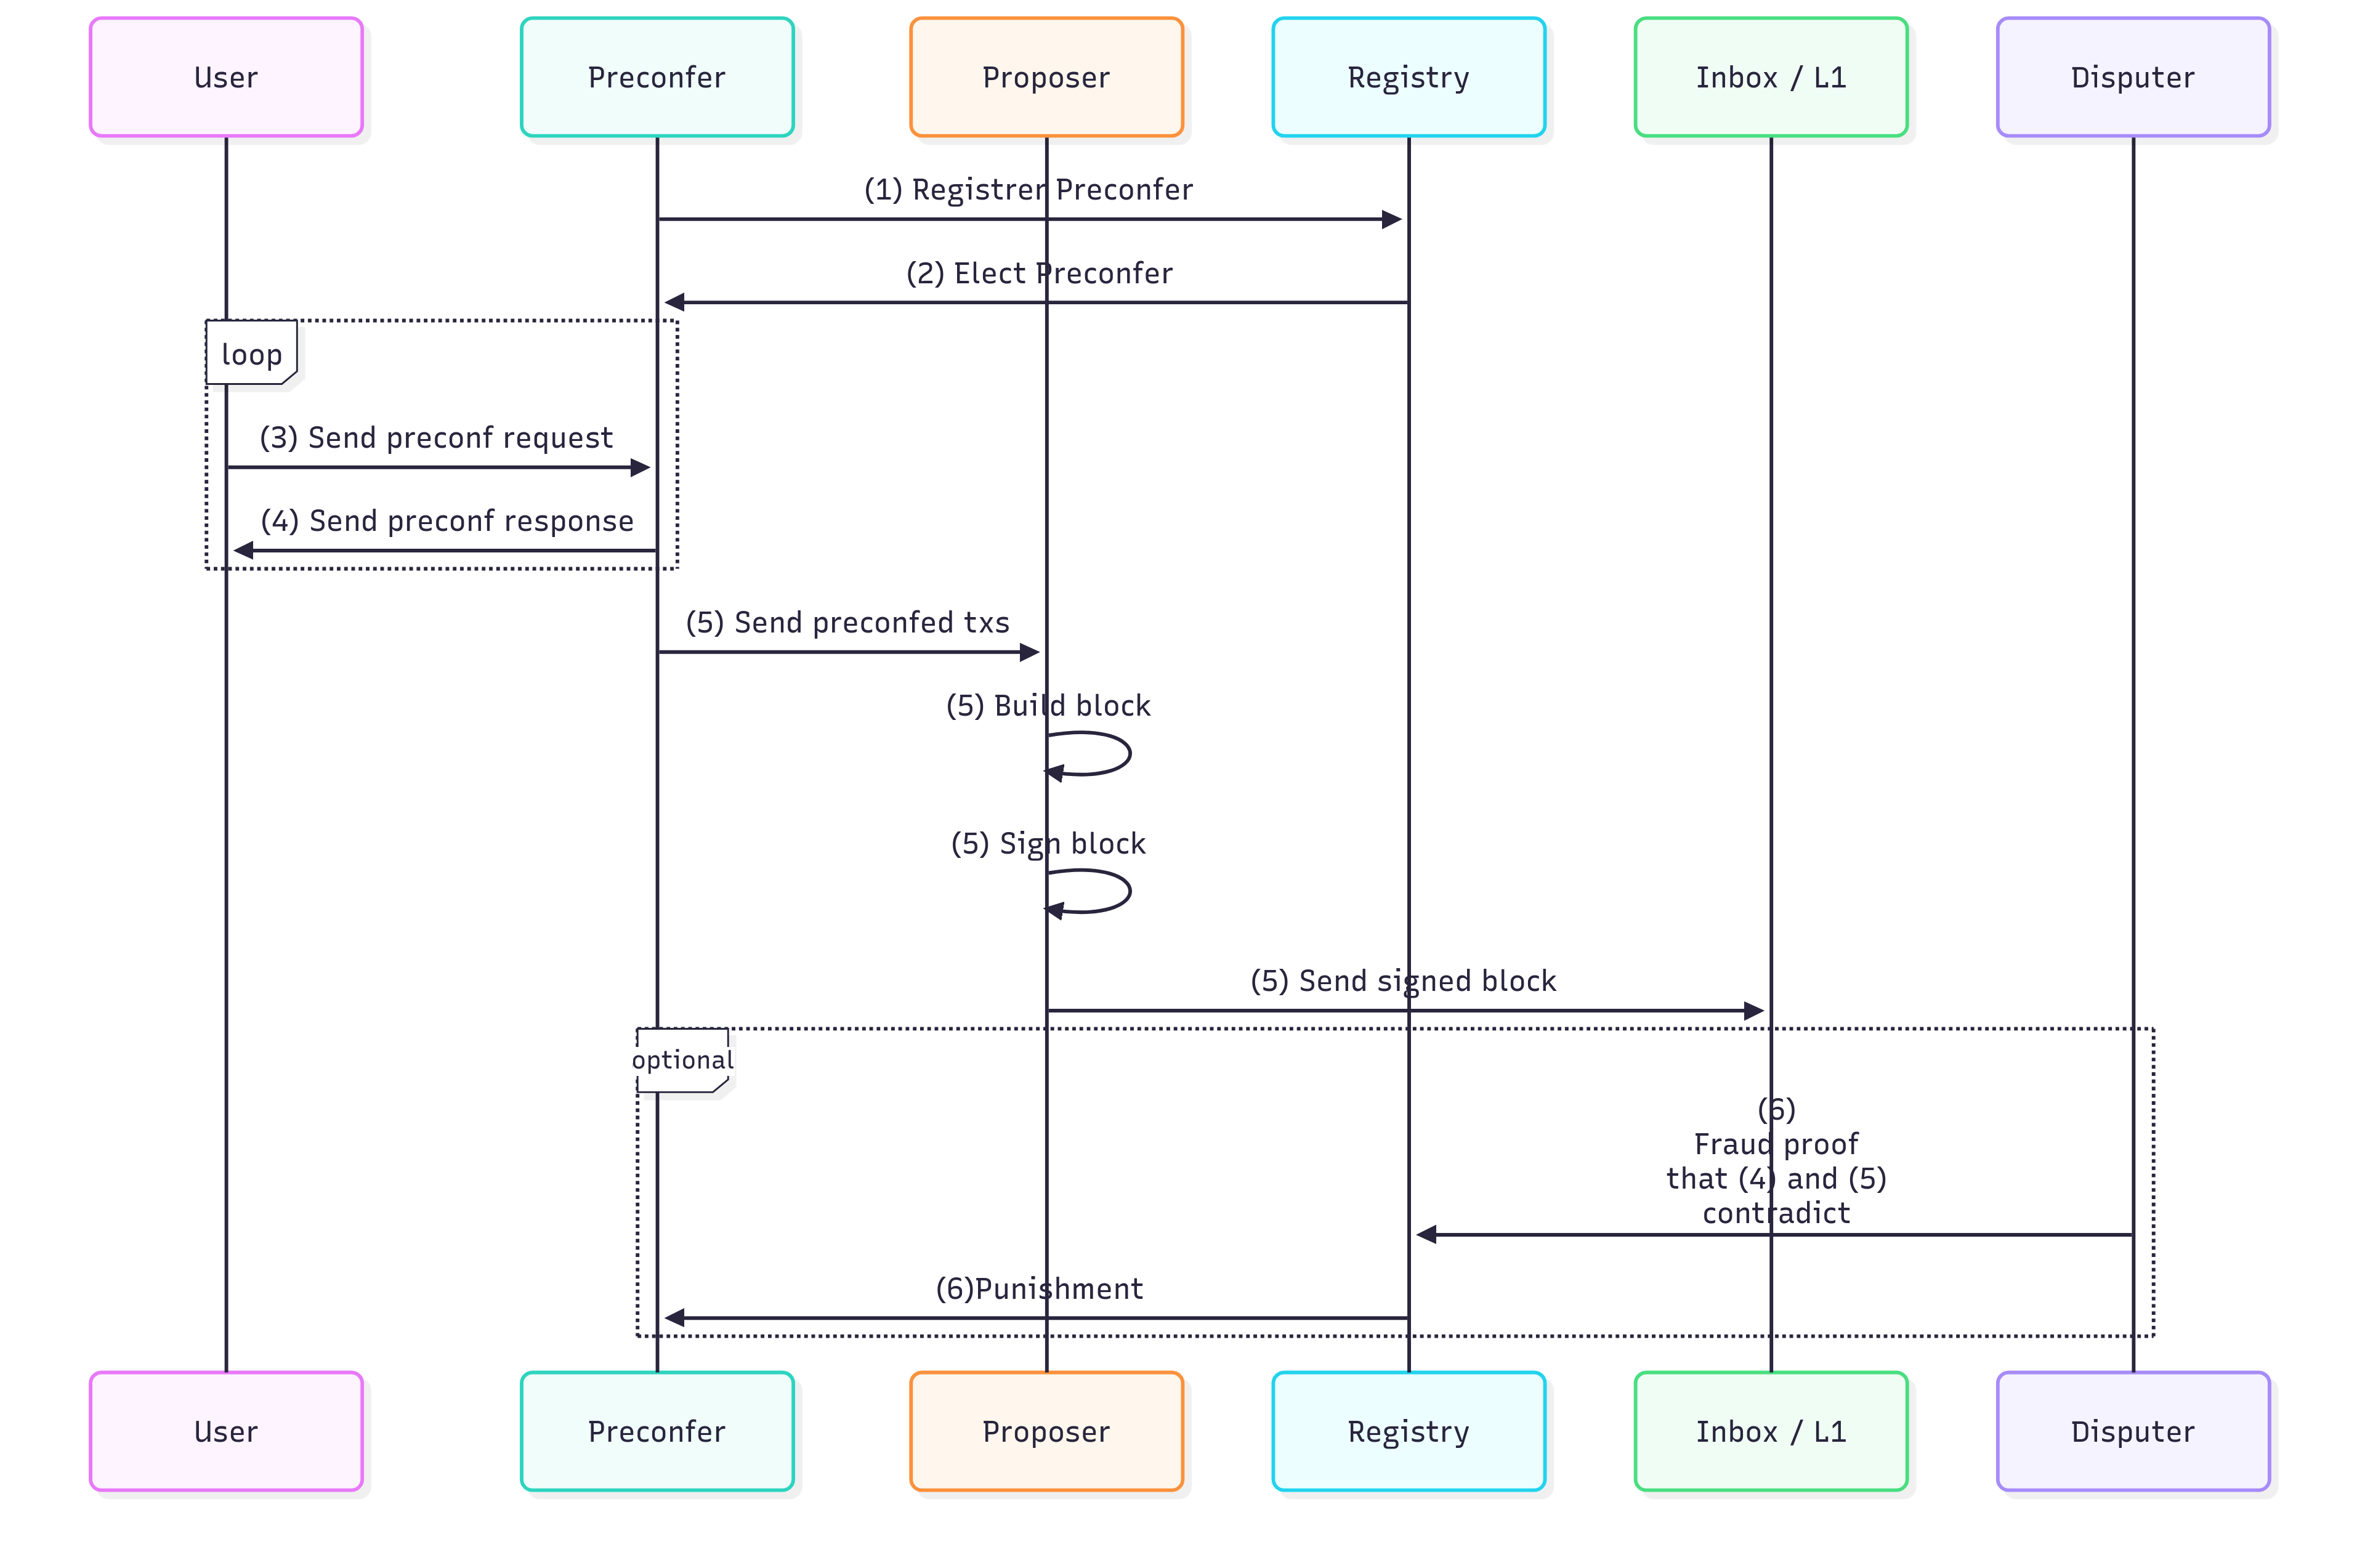
\includegraphics[width=0.9\textwidth]{figures/preconfProtocolFlow.png}
        \caption{Preconf protocol flow.}
        \label{preconf_protocol_flow}
    \end{figure*}
    \tododk{Update Disputer to Overseer?}
    
\subsection{Step 1: Preconfer Registration} 

\todo{consistency with 7.1; generalizable opt-in w.r.t slashable collateral}

\label{step1:preconfer_registration}
    The first step in our preconf protocol flow is preconfer registration (see \hyperref[preconf_protocol_flow]{Fig.~\ref{preconf_protocol_flow}}). Preconfer registration involves candidates signaling that they want to become a preconfer. For this signaling to result in a successful registration, the candidate must meet all applicable registration requirements/eligibility criteria. %\qb{should we pick one term?} \ks{i have retained both terms for now because we need both of them in different sections.
    Each preconf registry has the freedom to set its own criteria for its preconfers. Some example criteria include:
    \begin{itemize}
        \item Proof that a registrant is a proposer. Generally, preconfers must have the ability to perform inclusion/execution of a preconfirmed transaction. Some preconf protocols may insist that preconfers be proposers of the underlying blockchain protocol. Specifically, registrants may need to prove:
        \begin{itemize}
            \item Membership of the L1 proposer set for L1 and based L2 preconfs.
            \item Governance committee approval for non-based L2 preconfs.
        \end{itemize}
        \item Deposit of some minimum collateral amount that may be subject to slashing~\cite{W:CrediblyNeutralPreconfirmationCollateral:ThePreconfirmationRegistry, W:PreconfirmationRegistry}.
        \item That a registrant is not blacklisted cf. \cite{W:PreconfirmationFairExchange}.
        \cm{i deleted "belonging to a whitelist", as the whitelist is the registration.}
        
    \end{itemize}

        \subsubsection{The Preconfer Registry} \label{preconfer_registry}
        \todo{add section intro text}
        \begin{definition}
            In the context of preconfs and a specific preconfer, \textbf{slashable collateral} is an amount of tokens that can be slashed in the case of that preconfer's misbehaviour. 
        \end{definition}
        \todo{add connective text}
        
        \begin{definition}
\label{def: preconf_registry}
        A \textbf{preconfer registry} is a smart contract wherein entities can opt in to preconfing, registering themselves as preconfers. This smart contract can: (i) verify whether a candidate meets the applicable eligibility criteria; (ii) hold collateral and enforce monetary penalties on preconfers deemed to have acted maliciously in accordance with contract rules; and (iii) determine the preconfer schedule.
        \end{definition}

        
        Preconfer registries \cite{PreconferRegistryArticle,W:UniversalRegistryContract} can play an important role in their respective blockchains. For L2s, preconfer registries can be tightly coupled with the proposer election mechanism, including having full control over proposer election.\footnote{For more details, see Section \ref{preconf_election}}.\todoks{Consistency with forward referencing here}
 
        Preconfer registries where proposers can opt-in to preconfing are expected to require preconfers to deposit some slashable collateral. In such protocols, the preconfer registry would be entrusted to manage the collateral on behalf of preconfers. This includes slashing of the collateral when deemed necessary by any registry-specified rules, known as slashing conditions\cite{W:Documentation-RegisteringasaProvider,W:PreconfirmationRegistry}. 
        These slashing conditions should in theory reflect the behaviours that are desired/acceptable from a preconfer. As such, the threat of losing some or all slashable collateral as a result of violating a slashing condition can act as a deterrent to dishonest preconfer behaviour. Slashing of collateral, and alternative punishment methods are thoroughly discussed in \hyperref[preconfer_punishment]{Section~\ref{preconfer_punishment}}.  \todoks{Consistency with forward referencing here}
         
        Note that any preconfer collateral directly locked up in a preconfer registry cannot be reused for other purposes. Therefore, protocols may want to rely on third-party restaking platforms for sourcing slashable collateral, such as the EigenLayer platform~\cite{W:RestakingOverview}. Restaking allows collateral to be reused for multiple purposes, making it an attractive capital-efficient means for sourcing collateral. Of course, repurposing slashable collateral for multiple protocols introduces risks related to stake being slashed in multiple protocols at once. This risk reduces the per-unit security of restaked collateral compared to single-use collateral deposited directly to a preconfer registry. For more information on these trade-offs, see \cite{W:Restaking101:APrimeronEigenLayer}.
        
        \par 
        
        Lastly,  in an attempt to make preconfirming accessible to solo-stakers with limited resources, \qb{think we can integrate the reference better} \todoqb{what do you suggest here? - happy now; we needed/need consistency between "in [x], the authors... / [x] shows how...; not a fan of either unless doing a literature review. Current form is fine.}, collateral delegation has been proposed \cite{W:CrediblyNeutralPreconfirmationCollateral:ThePreconfirmationRegistry}. Collateral delegation allows delegates to delegate stake to a delegatee who wishes to act as a preconfer but does not possess the required collateral. In such a setting, if a delegatee violates a slashing condition, it would be the delegates' stake that would be slashed. Sharing of preconfer rewards would be one reason for delegating collateral, although delegation comes with significant risk for delegates.

        \paragraph{Universal Registry Contract}
        At the time of writing, all preconf protocols implement and deploy their own standalone registry contract. The ``Universal" Registry Contract  (URC)~\cite{W:UniversalRegistryContract,W:GitHub-UniversalRegistryContract} aims to address the fragmentation risks that standalone preconfer registries inherit. The URC aims to be a generic, open-source contract that removes the need to create an maintain individual preconfer registry contracts for each preconf protocol. The URC's promise is that individual protocols can customize their slashing and collateral requirements outside of the core URC. The URC aims to standardise:
        \begin{itemize}
            \item Preconfer registration and collateral posting.
            \item How slashing condition violations are reported and enforced. Specifically, the URC aims to create a common language and proving methodology for slashing conditions.
            %For example, the proof may include the preconfirmation response  stating that the preconfer will pay 1 ETH if they fail to include the transaction in the next block, along with evidence that the transaction was indeed omitted from that block.
        \end{itemize}

        With a single shared preconf contract like the URC, there is an easier path for preconf adoption for all stakeholders. If collateral amounts, slashing conditions, and violation reports have a common language, the adoption of preconfs becomes greatly simplified. By having one preconfer registry instead of many to understand and audit, the sophistication requirement of stakeholders is greatly reduced, which is crucial for mass adoption. One preconfer registry simplifies the tasks of assessing and comparing preconf protocols, slashing conditions, preconf guarantees and preconf risks  (see Section \ref{sec:risk}) \cite{W:CrediblyNeutralPreconfirmationCollateral:ThePreconfirmationRegistry}) \tododk{KS: I did not find in this source a mention to UCR. Maybe we need here another reference?}. %For more details about the ``universal" registry contract cf. \hyperref[registry_implementations]{Section~\ref{registry_implementations}}).


      
\subsection{Step 2: Preconfer Election} 
\tododk{Dimitris, Lin please take a look at the missing references.}
\todolo{Dimitris, Lin please take a look at the missing references.}
\label{preconf_election}

Preconfer election is a crucial part of most preconf protocols
This section examines how preconfers are elected.
As already mentioned, in many L2s, the preconfer registry and proposer election are aware of each other, and in some cases, they are the same smart contract \cite{Optimism,ZKsync,Arbitrum} \todolo{ add Taiko whitelist link}. In contrast, L1s and based L2s are not typically aware of the preconf registry, or even that preconfs are taking place. In all cases, the preconfer registry must be consulted to identify the schedule of preconfers, and for what slots preconfs can be provided. Thus, the way the next preconfer is elected by the preconfer registry depends on (i) the type of the preconf (inclusion or execution), and (ii) the underlying blockchain and how this blockchain elects proposers.

\paragraph{How Inclusion vs Execution preconfs affect preconfer schedule}

If the current proposer of a blockchain is not a preconfer, then execution preconfs cannot be credibly provided, even if future proposers in the proposer lookahead are preconfers. This is because the current proposer has control over the next blockchain ledger update, and as such, future preconfers cannot know the blockchain ledger on which they will act.
\chm{How does this fit with builders as preconfers?}

On the other hand, inclusion preconfs can be issued by many, if not all preconfers. This is because the fulfillment of inclusion preconfs does not depend on the current state of the blockchain ledger.  


\paragraph{ How the type of the blockchain affects preconfer schedule}
\begin{itemize}
    \item \textbf{L1 and based L2s}: Proposers are determined via the L1 proposer election mechanism. L1 preconfer registries -- while not responsible for electing L1 proposers -- can still determine the preconfer schedule, e.g. through EIP-7917~\cite{EIP7917} \todoks{examples consistency}. The preconfer schedule can be determined by finding the intersection of the registered preconfer set and the proposer lookahead, and taking into account whether the preconf is inclusion or execution.
    \item \textbf{Non-based L2s}: Within non-based L2s, there is a large proposer-preconfer election design space. The preconfer registry can either read from the outputs of a standalone proposer election mechanism as in L1 and based L2 preconfs, or be integrated into the proposer election mechanism ~\cite{, Optimism, Arbitrum, ZKsync, Starknet}. \tododk{Dimitris, we need a reference for non-based L2s}
\end{itemize}

\tododk{KS: assign the following citations to the correct bullet above \cite{Optimism, Arbitrum, ZKsync, Starknet}? We removed them from section 4, so we need to add them here}
There is an interesting preconfer election design for L2s that is not perfectly handled by the above categorizations which is seeing active consideration \todolo{post whitelist Taiko reference? anything else}. In this design, L2 proposers must be registered as preconfers. L2 proposers are selected from the L1 proposer lookahead, as in based L2s, except when there is no registered preconfer in the L1 proposer lookahead. In this case, the L2 proposer is selected from the preconfer registry. This categorization looks somewhat like our categorization of based L2s, apart from the scenario where no registered preconfer exists in the proposer lookahead.


\subsection{Step 3: Preconf Request} \label{preconf_request}
    As soon as a registered preconfer is elected, users who wish to receive preconfs can begin submitting preconf requests (see \hyperref[preconf_protocol_flow]{Fig.~\ref{preconf_protocol_flow}}). Depending on the protocol, users can route preconf requests to the preconfer via P2P~\cite{W:Documentation-Understandingmev-commit} or through RPC endpoints~\cite{W:Taiyi-off-chaincomponents,W:Towardsanimplementationofbasedpreconfirmationsleveragingrestaking}. The request structure can vary from protocol to protocol. Preconf requests may include the following:


    

    \begin{itemize}
        \item \textbf{Transaction(s):} Requests are expected to include the transaction(s) for which the user wishes to receive a preconf. \footnote{Other preconf protocols allow users to request intent fulfillment \cite{W:Intent-BasedArchitectureandTheirRisks} or ahead-of-time commitments to include a transaction where the executable transaction has not been specified yet ~\cite{W:Proposer-CommitmentInfrastructureinEthereum,W:OpportunitiesandConsiderationsofEthereumsBlockspaceFuture, W:BlockspaceFutures}. These latter preconfs are sometimes referred to as block-space commitments}. 
        \item \textbf{Preconf tip:} The preconf tip is the compensation to be paid to the preconfer for the preconf. In some protocols, the tip is atomically bundled with the transaction that requires inclusion preconfirmation. This means that the preconfirmer cannot redeem the tip without including the transaction (cf. \cite{W:TheDerivationPipeline}) \todoks{reference consistency} \tododk{Dimitris could you please add also the following citation here?  \url{https://ethresear.ch/t/analyzing-bft-proposer-promised-preconfirmations/17963}}. 
        However, it is likely important that a preconfer does not receive a preconf tip if the preconfer fails to honour the preconf's predicate. 
        %It is atomically binded to the tx so the preconfer cannot redeem the tip without honouring the preconf \lo{Not sure if it has to be atomically bound. For example, you can have non-atomically-bound tip but quick preconfs enforced via fair exchange solution. In a sense, centralized seq can be thought of doing this.}. 
        The preconf tip is a key incentive for preconfers to provide preconfs. As such, pricing models for preconf tips are crucial. Preconf tip pricing is handled in detail in \hyperref[EconomicViabilityOfPreconfs]{Section~\ref{EconomicViabilityOfPreconfs}}. \todoks{internal reference consistency+ we need to check later this link}
        % \cm{finish with something like: pricing is handled in detail in later Section, Section ABC}
        % \cm{for the final document, it doesn't make sense to me to go off topic for the next paragraph and talk about calculating tips. I think this is part of incentives/MEV section which should be later in the doc}
        % However, calculating a sufficient tip is non-trivial and can be very challenging. Preconfers are required to solve an online MEV problem and decide whether to accept or reject a preconf request without having a complete image of all the potential txs they can include in the block. This means that the tip should be alluring enough to make the preconfer commit to including/executing a tx instead of rejecting it for the possibility of increasing MEV later within the slot. Subsequently, the preconfer has a motive to delay responding to requests in order to maximise MEV which leads to the fair-exchange problem that will be further investigated in the next paragraphs~\cite{W:StrawmanningBasedPreconfirmations}. \cm{this comment is referring to what paragraphs? I don't see the logical next here} \qb{agreed}
        
        \item \textbf{Preconf type:} 
        % \cm{why doesn't preconf type need to be specified by all} \qb{I think because the section starts with the idea that the user signs a request that contains some parameters, but the actual type of preconf requested can in some protocols be deduced from the structure of the preconf request itself, hence it doesn't need to be specified (don't recall exactly which article it was, just remember reading it)}
        Provided that the protocol and/or the preconfer support both inclusion and execution preconfs, users should specify which type of preconf they want.
    \end{itemize}

    Requests may also contain more nuanced parameters:
    \begin{itemize}
        \item \textbf{Deadline:} A deadline parameter sets the latest possible slot/time after which a request should be considered void, and its transaction(s) no longer includable by the preconfer~\cite{W:PreconfirmationsforVanillaBasedRollups}. 
        
        \item \textbf{Tip decay/escalator mechanism:} 
        The preconf tip may need to change during the duration of a request to reflect a request submitter's urgency for a preconf to be fulfilled. A tip decay or escalator mechanism can achieve this. Tip decay mechanism can incentivize individual preconfers to respond in a timely fashion to maximise the tip receive\cite{W:Documentation-BidDecayMechanism}. Tip escalators have also been discussed for regular transactions in \cite{W:OrderflowauctionsandcentralisationII:orderflowauctions}. Tip escalators depend on multiple entities competing to act on a transaction or preconf at the same time. This means such a mechanism would be more appropriate for inclusion preconfs, or execution preconfs from builders.   
        
        \item \textbf{Preconf penalty:} Instead of relying on a predetermined penalty system, it is possible that users define penalties for preconfer faults related to a specific request through a request parameter~\cite{W:User-DefinedPenalties:EnsuringHonestPreconfBehavior, W:Documentation-BidStructure}. The idea is to allow users and preconfers to mutually agree on a level of cryptoeconomic security where a ``one-size-fits-all" approach does not suffice.
        
        
        \item \textbf{Latest preconfirmed state}: 
        It is possible for protocols to allow users to specify a commitment to the latest blockchain ledger, concatenated with any transactions that have already been preconfirmed since the last ledger update.\chm{Hard to understand.} This gives users control over the transaction sequence their request acts on.  ~\cite{W:AnalyzingBFTProposer-PromisedPreconfirmations}

        
        \item \textbf{Privacy preferences:} 
        Privacy-preserving techniques may be applied to preconf requests to hide key request data from block proposers before they issue the preconfirmation %(e.g. \cite{W:PreconfirmationsundertheNOlens}). 
        Techniques include public-key encryption, or trusted intermediaries as are used in MEV-Boost works today~\cite{W:BasedPreconfirmationswithMulti-roundMEV-Boost, W:AnalyzingBFTProposer-PromisedPreconfirmations, W:Documentation-BidStructure, W:Towardsanimplementationofbasedpreconfirmationsleveragingrestaking}. % unwanted entities in the block-building pipeline \qb{are there "unwanted entities" in the pipe-line? perhaps untrusted fits better?}, including some subset of preconfers, or even from preconfers themselves until a response is provided. Techniques include public-key encryption, or trusted intermediaries as are used in MEV-Boost works today~\cite{W:BasedPreconfirmationswithMulti-roundMEV-Boost, W:AnalyzingBFTProposer-PromisedPreconfirmations, W:Documentation-BidStructure, W:Towardsanimplementationofbasedpreconfirmationsleveragingrestaking}.
         
    \end{itemize}
    
    
\subsection{Step 4: Preconf Response} \label{preconf_response}
      
    After observing a preconf request and verifying its validity, the preconfer must then choose whether to provide a preconf or not. This section describes the process of responding to preconf requests. Generally, preconfers should be incentivised by the protocol to provide timely responses to users in order to improve UX. To incentivize timely responses, we require a suitable tipping mechanism (as discussed in Sections \ref{preconf_request} and \ref{sec:price}), along with a protocol that ensures the preconfer receives the tip only if the preconf is provided no later than the agreed-upon time (as discussed in Section \ref{fair_exchange_problem}.) \todoks{consistent internal referencing}
    \chm{It seems a preconf response is the preconf. The term ``response'' suggests it is something given in reply to a preconf.}
    
    Responding to a preconf request binds the preconfer to a commitment to include or execute the preconfirmed transaction. In many protocols, preconf responses also serve as evidence for punishing dishonest preconfers who fail to fulfill stated commitments (cf. URC described in Section \ref{URC}). \todoks{consistent internal referencing} 
    Preconf responses must be signed by the preconfer. Additional, responses may include (but are not restricted to):
    \begin{itemize}
        \item \textbf{Unique identifier to a preconf request:}
        A response must contain a unique mapping to the request it is directed at. A hash of a signed request is such a mapping~\cite{W:Documentation-Commitments}.
        
        \item \textbf{Block number containing the requested transaction or validity period:} Some preconf protocols may require the preconfer to disclose the number of the block that will contain the requested transaction, or commit to the period during which the preconfirmation will be fulfilled~\cite{W:Towardsanimplementationofbasedpreconfirmationsleveragingrestaking}.

        \item \textbf{ Latest preconf state:}
        The preconfer may be required to provide a commitment to the updated preconf state (explained in the preconf request Section) \todoks{appropriate interal reference here.} at the instant when the preconf response was provided. 
        
        \item \textbf{Commitment to additional slashing conditions:} Certain preconf protocols may require a preconfer to commit to additional slashing conditions -- for example, as specified by the associated preconf request. \todoks{example referencing}
        \item \textbf{Timestamp:} The time at which the preconf response was issued.
        
    \end{itemize}

    Apart from the content of a preconf response, the frequency of preconf responses can also vary. Preconf responses can be published in several ways:
    \begin{itemize}
        \item Immediately upon commitment to fulfill the preconf (streaming) \url{https://ethresear.ch/t/the-preconfirmation-gateway-unlocking-preconfirmations-from-user-to-preconfer/18812} \todoks{add reference}
        \item At regular time intervals
        \item In batches -- for example, after every ten responses \chm{This is confusing. A response is only given after every ten responses? Then no response is ever given.} \todoks{consistency with examples}
        \item Upon request, granting access to previously issued responses
    \end{itemize}
    \todoks{Conor added a new paragraph to separate response formatting from preconf timings. Please review.}
    The frequency with which preconf responses are expected, enforced, and actually provided has implications for all stakeholders of a preconf protocol. For example, streaming preconfs is resource intensive for a preconfer, both from an infrastructure and a pricing perspective (see Section \ref{sec:price} for more details on how response frequency affects preconf pricing and preconfer revenue). On the other-hand, streaming preconfs likely offer an improved user experience compared to alternatives.
    

\subsubsection{Fair-Exchange of Preconf Requests and Responses} \label{fair_exchange_problem}
    Equally important to the core concepts of requests and responses is the fair exchange of requests and responses. 
    \begin{definition}
        
    The \textbf{fair exchange problem} states that during a mutual exchange of items between two parties, it is vital to guarantee that both parties or neither party receive the expected item. No party should have the ability to gain an advantage by misbehaving or quitting the transaction prematurely~\cite{P:Fairexchangewithasemi-trustedthirdparty,T:Fairnessinelectroniccommerce}.
    \end{definition}

    In the context of preconfs, users should have some expectation of how and when responses are received after submitting a request. This expectation depends on many factors, including but not limited to the type of preconf, the tip being paid, the cost to provide and fulfill the preconf, the relative demand for transactions/preconfs at the time the request was sent, and the value that a preconfer can extract from the preconf beyond the tip. Crucially, a preconf user's expectation has a time component built in -- users typically want preconfs sooner rather than later. This makes the fair exchange of preconfs more complex than eventual fair exchange of request and response. \cite{W:PreconfirmationFairExchange} introduces the concept of timely fair exchange to explain this user preference in the context of preconf protocols. Previous work on fair exchange proved that it is impossible to enforce fair exchange without a trusted third party~\cite{P:OntheImpossibilityofFairExchangewithoutaTrustedThirdParty}. As such, preconf protocols need to introduce some form of trusted third party in order to provide meaningful guarantees of timely fair exchange. \chm{Can't a smart contract on the blockchain be the trusted third party?}
    
    \begin{definition}
    \label{def:overseer}
    In the context of preconfs, an \textbf{overseer} is an entity or set of entities that is trusted to observe the actions of preconfers, and provide signals to the protocol in the case of a preconfer's deviation from protocol rules or expected actions. These signals can include proofs of deviation, although some deviations may not be provable, depending instead on overseer trust. Overseer signals may be communicated on-chain through protocol smart contracts, or off-chain through P2P communication layers.
    \end{definition}

    Several overseer election mechanisms have been discussed. The primary distinction of these protocols is based on whether the overseer can signal preconfer misbehaviour in-protocol or not. In-protocol signaling allows for explicit preconfer punishment, something which is discussed in \hyperref[preconfer_punishment]{Section~\ref{preconfer_punishment}} \todoks{internal ref}.
    Such overseers can be elected through governance, and/or be required to hold some large amount of a blockchain's native token for which the preconfs are being provided. Both of these mechanisms align overseers with the success and reliability of the preconf protocol. 
    
    For overseers who are expected to signal preconfer deviation out-of-protocol, several solutions have been discussed to date. In \cite{W:PreconfirmationFairExchange}, users are collectively identified as a suitable overseer in certain preconf protocols. Users can use the threat of withholding orderflow from a misbehaving preconfer to incentivize preconfers to follow protocol rules. The effectiveness of orderflow withholding as a threat depends on the expected profit of a preconfer from preconfs. This in turn is influenced by the frequency of being elected as a proposer/preconfer and the availability of block space (cf. \cite{W:Future-ProofingPreconfirmations}).
    %is greatest when there is a single preconfer for the duration of the protocol, as in single-proposer L2s. For every additional preconfer added to the preconfer set, the effectiveness of orderflow loss is diminished proportionally to the number of preconfers; if a preconfer only has access to orderflow once every $N$ slots in expectation, the threat of orderflow loss for that preconfer is $1/N$th of the threat in the single preconfer case. As such, if possible, elected overseers should be favoured over users to enforce timely fair exchange of preconfs with a large/permissionless set of preconfers. 
    
    Wallet providers operating as out-of-protocol overseers on behalf of users is also discussed in \cite{W:PreconfirmationFairExchange}. As wallet providers are more sophisticated than a typical blockchain user, wallet providers may be better suited to identify preconfer deviations.
    In a similar vein, \cite{W:ThePreconfirmationGatewayUnlockingPreconfirmations:FromUsertoPreconfer} presents the concept of gateways \ks{(cf. Def. \ref{def:preconfirmation})} \todoks{internal ref} relayers (cf. \ref{sec:L1_pipeline}) acting as overseers on behalf of users by monitoring preconfer behavior and withholding requests or tips. However, as gateways and relayers are also being considered as preconfers, alternative overseer solutions must also be considered. 
  \ks{Conor I think that the last sentence need rephrasing because in Definition 6 and section 5.5 we use the  term gateway for every entity that issues preconfs on behalf of proposers }  

\subsection{Step 5: Fulfillment }\label{preconf_delivery}

\tododk{need to link proposer and preconfer to comply with the diagram}


It is a preconfer's ability to fulfill a preconf that provides a preconf protocol with utility. This section focuses on the different mechanisms that preconfers can use to fulfill preconfs. These fulfillment mechanisms depend on many factors, including but not limited to:
\begin{itemize}
    \item What layer of blockchain the preconfs apply to.
    \item How much of a block is being preconfed, and how any remaining blockspace is filled when only a percentage of a block is being used for preconfs.
    \item Whether the preconfer is a proposer or gateway.
\end{itemize} 
These tradeoffs are examined in the following Fulfillment Tradeoffs subsections.

\subsubsection{Fulfillment Tradeoffs: Based vs Non-Based}

For L1 and based L2 preconfs, the L1 proposer controls proposal of L1 blocks, and so can always propose an L1 block containing any and all preconfs. For non-based L2s with a single proposer, fulfillment is also controlled by the proposer themselves. 

In the case of non-based L2s with mutliple proposers, the rules of the underlying L2's blockchain ledger dictate a preconfer's ability to fulfill preconfs. In some non-based L2s, it may be sufficient to just propagate the block to the P2P layer for consensus. However, some non-based L2s require that an L2 proposer's blocks must appear in the L1 ledger by a certain proposal deadline to be considered valid. In this case, an L2 preconfer can only fulfill their preconfs if an L1 proposer includes the corresponding L2 blocks on L1 by the proposal deadline, which is not guaranteed. 

\subsubsection{Fulfillment Tradeoffs: Full Block Preconfs vs Partial Block Preconfs}

In the case where a full block is being used for preconfs, a preconfer can build the block themselves and ensure fulfillment of all preconfs. In the case where only a partial block is used for preconfs, and the final block is built at proposal time, potentially including non-preconfs, there must be a mechanism in place to ensure the final block satisfies all preconfs. A simple algorithm for achieving this is including all preconfed transactions first in a block, followed by the remainder of the block. However, when any of these preconfed transactions are inclusion preconfs, this simple algorithm is likely sub-optimal for a proposer with regard to capturing block-building revenue. As inclusion preconfs can be placed anywhere in a block, a proposer can strategically place these preconfs to maximize their MEV revenue. 

That being said, this problem of maximizing the value of blocks given some constraints has parallels to the ordered knapsack problem ~\cite{P:Partiallyorderedknapsackandapplicationstoscheculing}, which requires significant sophistication to solve for the knapsack sizes and number of items that modern blockchains provides. This problem has been terms \chm{Typo?} the Online Block Packing problem \cite{OnlineBlockPacking}. To allow proposers to outsource this complex optimization problem while still receiving revenue from the solution, the Constraints API~\cite{W:ConstraintsAPISpecification} has been proposed as a tool to allow proposers to offer preconfs (or apply arbitrary constraints on a block), and then outsource the building of a block satisfying all preconf predicates to a set of builders, analogously to how proposers outsource building through MEV-Boost \cite{MEV-Boost}. 

\subsubsection{Fulfillment Tradeoffs: Proposer vs Gateway}
\label{delivery_tradeoffs}

Proposers are perfectly placed to provide preconfs, given their ability to include preconfs in their own blocks. Gateways on the other hand require additional machinery to ensure that a proposer proposes a block which includes all preconfs provided by the gateway. The relationship between the proposer and gateway is crucial to the mechanism that must be used to fulfill gateway preconfs. 

If the gateway trusts the proposer, a straightforward message-passing algorithm suffices to fulfill preconfs from gateway to proposer to the blockchain ledger. Depending on whether or not the gateway is also tasked with sourcing the block for the proposer will dictate the time at which the preconfs must be sent back to the proposer, or whether the proposer even needs to observe the preconfs. In the case where the gateway also sources the proposer's block, for example if the gateway also runs MEV-Boost, the proposer can simply sign the block header and have the gateway propagate the final block to the P2P network, as in MEV-Boost.

If a gateway does not trust a proposer, the gateway would require cryptoeconomic guarantees that the proposer will propose a block that includes all preconfs provided by the gateway. Cryptoeconomic guarantees from the proposer are especially important when the gateway is liable to be punished in the case where preconfs are not fulfilled. Such a guarantee could include shared punishment when preconfs are not fulfilled, or the existence of a mutually trusted overseer to arbitrate faults \cite{W:PreconfirmationFairExchange,W:FaultAttribution}. 

In \cite{gateway_trust_liveness}, it is proposed to penalise entities based on the specific reason a preconf was not fulfilled. If no block was published for the relevant slot, the proposer is penalised. Conversely, if a block was proposed but the preconf was still not fulfilled, the gateway is held responsible and penalised.


\subsubsection{Designing Robust Fulfillment Mechanisms}\label{robust_delivery}

    In any preconf protocol where preconfer rotation takes place \chm{Also possible if no rotation takes place.}, it is possible that a preconfer fails to fulfill their preconfs. Although this non-fulfillment may be malicious, non-fulfillment of preconfs can also be unintentional. Some thought has been given to protecting against unintentional failures to fulfill preconfs.
    
     The authors of \cite{W:AvoidingAccidentalLivenessFaultsforBasedPreconfs} suggest that preconfers can collaborate with subsequent preconfers through revenue sharing to preconf the same transaction sequences in the event that the original preconfer fails to fulfill the preconfs themselves. This approach is termed \textbf{chaining} preconfs. Although the exact incentives and guarantees of chaining are unexplored, chaining provides a protocol design direction to protect preconfers and their users from the risks of failing to fulfill preconfs. 
     
    
\subsection{Step 6: Preconfer Punishment} \label{preconfer_punishment}    
    \cm{this section is bigger than just punishment, I think the name needs to be slightly more general} \ks{Preconfer Faults and Punishments?}
    % tx(s)/intent/operation \dk{maybe we need a name for "tx(s)/intent/operation" to avoid writting the whole thing over and over again} \cm{maybe request is appropriate? We can make this connection in the request section if so.} was included or executed as specified by the preconf request and response. 
    Preconfer punishments are an important tool that can be utilised to incentivize or ensure that preconfers fulfill preconfs according to any restrictions set out by the protocol, a request, and/or a response.
    
    \subsubsection{Preconfer Faults} \label{preconfer_faults_and_punishing_conditions}
    There are various faults that a malicious or negligent preconfer can commit that jeopardise the smooth operation of a preconf protocol. Fig.~\ref{preconfer fault tree} presents a decision tree that categorizes preconfer faults. Preconfer faults are as follows:

    \paragraph{Safety Fault}
        \begin{definition}
            A \textbf{safety fault} occurs when the proposer publishes a block which violates a preconf predicate to which the preconfer committed.
        \end{definition}
        A safety fault will never be committed by an honest preconfer who is also a proposer. In such cases, the punishment is expected to be severe~\cite{W:Basedpreconfirmations}.
        
        
    \paragraph{Liveness Fault}

    \par
    Unlike safety faults, liveness faults are slightly different for L1s and based L2s compared to non-based L2s. We define liveness faults in the respective blockchains as follows:
    
        \begin{definition}
            A \textbf{liveness fault for L1 and based L2 preconfs} occurs when an L1 proposer does not publish an L1 block for a particular slot, meaning all preconfed transactions for that slot are not included in the respective blockchain ledger.
        \end{definition}
         \begin{definition}
            A \textbf{liveness fault for non-based L2 preconfs} occurs when the L2 proposer does not publish an L2 block to the P2P network, meaning all preconfed transactions for that slot are not included in the L2 blockchain ledger.  \end{definition}

        Unlike safety faults, liveness faults can be accidental and non-malicious, for example, due to a power outage or internet downtime. Therefore, protocols may prefer a lighter penalty for liveness faults \ks{(e.g.,~\cite{W:Basedpreconfirmations})} or introduce fulfillment mechanisms that mitigate the risk of preconfirmers being slashed for accidental violations, as discussed in \hyperref[robust_delivery]{Section~\ref{robust_delivery}}. \todoks{consistent internal mentions}      
        %That being said, from the perspective of the user, liveness faults can be indistinguishable from safety faults and may need to be punished severely~\cite{W:Basedpreconfirmations} \cm{this is a bold statement, so we need an example if this is true.}. 

            
        % To mitigate the punishments needed in the case of an accidental liveness fault, \cite{W:AvoidingAccidentalLivenessFaultsforBasedPreconfs} suggests a chained preconf system where following preconfers in the lookahead can honour a preconf that was not fulfilled by the active preconfer due to liveness failure. \cm{Introducing a protocol like this requires 1 or 2 more sentences so the SOK is self-contained. Why would the following preconfer chain preconfs? Any limitations to this chaining protocol?}
        
    
    %\paragraph{Condition Fault \dk{or Broken request conditions or parametric fault or Specification Fault or Constraint Fault}} \ks{ I would omit this, because for the case of txs that we examine these faults are included in the safety faults (I have amended safety faults to include them). For example here \cite{W:Basedpreconfirmations} they define safety faults as ``A promise safety fault occurs when the preconfer’s slot was not missed and the promise is inconsistent with preconfed transactions included onchain." If we agree to omit it we need to update the image to remove it also from there. Lin is it ok?}
        %\begin{definition}
            %A \textbf{condition fault} occurs when a preconfirmed tx is included on-chain but the preconfer fails to comply with the conditions specified in the preconf request and agreed upon in the preconf response.
        %\end{definition}
            
        %As explained in \hyperref[preconf_request]{Section~\ref{preconf_request}}, users can set various parameters in their preconf request. If the preconfirmed tx(s) is included or executed, but without complying with the conditions set by the user, the preconfer should be liable to punishment~\cite{W:DelegationinBolt:OutsourcingSophisticationWhilePreservingDecentralization}.
        
    \paragraph{Idleness Fault}
        \begin{definition}
            An \textbf{idleness fault} occurs when a preconfer receives valid preconf requests but neglects their duty and fails to provide preconf services.
        \end{definition}
       Although idleness faults are not well-documented, it is natural for some preconfirmation protocols to require and enforce that preconfers issue preconfs under certain conditions, e.g., preconfing all valid requests, or preconfing all requests paying tips greater than a certain amount.
            
        As illustrated in Section~\ref{preconf_response} and Section~\ref{sec:price}, there are various factors that can influence a preconfer's decision to provide a preconf, such as the preconf tip and the incompatibility of conflicting transactions. As idleness faults depend on requests being delivered to the preconfer but not being responded to, this introduces a subjective observability requirement that could potentially be handled by a trusted party such as an overseer as presented in Section \ref{fair_exchange_problem}, Def \ref{def:overseer}).
        
        %As illustrated in \hyperref[preconf_response]{Section~\ref{preconf_response}} and \hyperref[EconomicViabilityOfPreconfs]{Section~\ref{EconomicViabilityOfPreconfs}}, \dk{this should be adjusted to point to preconf pricing}, there are various factors that can influence a preconfer's decision to provide a preconf, such as the preconf tip and the incompatibility of conflicting txs. Therefore, idleness faults can be handled by an overseer \cm{if not handled by an overseer, who else can handle this? Personally, I think we can say something stronger "likely need to be handled"}.

    \begin{figure}[htbp]
        \centering
        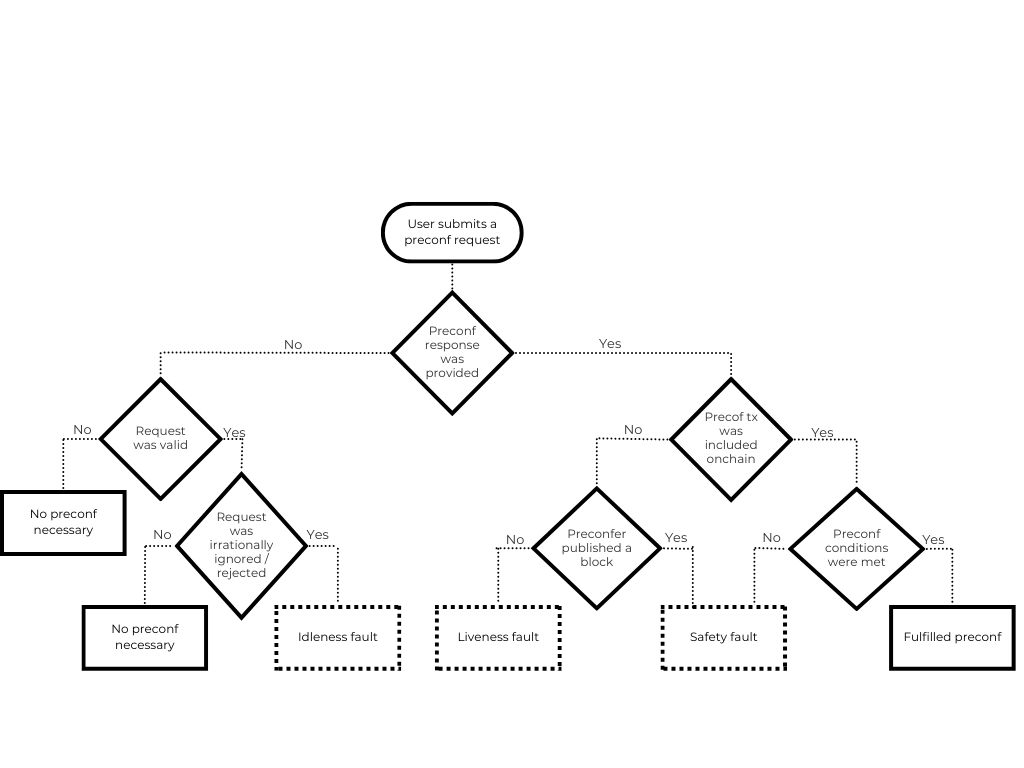
\includegraphics[width=0.9\textwidth]{figures/preconferFaultDecisionTree.png}
        \caption{Preconfer fault decision tree.\chm{Typo ``precof''}\chm{Preconfer may not be the one who publishes the block if not proposer.}}
        \label{preconfer fault tree}
    \end{figure}
    

\subsubsection{Enforcement Mechanisms and Proofs of Malicious Behaviour}
\label{sec:enforcement}

    \cm{EM abbreviation should be removed if only used several times}
    Preconf protocols rely on some form of economic incentives to encourage honest preconfer behaviour. These incentives are provided by mechanisms that either explicitly or implicitly punish malicious preconfer behaviour. 
    \begin{definition}
    \label{def:enforcement}
        An \textbf{enforcement mechanism} (EM) 
        triggers punishment of a preconfer when the preconfer satisfies one or more punishing conditions. 
    \end{definition}

    \todocm{Please review changes in this section - Q}

    There are many possible EM implementations. Key differences between EMs include whether the overseer responsible for observing punishing conditions is permissionless or permissioned, the type of proof required to trigger preconfer punishment, and the level of punishment~\cite{W:PreconfirmationFairExchange}.

    In a permissioned overseer setting, observation and triggering of punishments are driven by the permissioned overseer. Generally, the proofs required to initiate punishment for permissioned overseers are less rigorous.  Punishing conditions do not necessarily need to be proven to be satisfied, potentially only requiring an overseer signature. When proofs are not required to trigger punishments, this raises concerns about overseer abuse~\cite{W:PreconfirmationFairExchange}.

    In a permissionless setting, anyone can act as an overseer to initiate punishment via an EM. Contrary to the permissioned setting, permissionless overseers must be required to submit conclusive and indisputable evidence to trigger explicit preconfer punishments via the EM. Such evidence may include a signed preconf request, response pair disagreeing with the blockchain ledger. When indisputable evidence is not available, some form of arbitration between preconfer and overseer(s) must take place. As triggers are disputable in this case, this exposes permissionless overseer EMs to incorrect or unsatisfactory triggering and punishment~\cite{W:GitHub-UniversalRegistryContract,W:GitHub-ExampleSlasherImplementations,W:PreconfirmationFairExchange}. 
    
    Another important aspect related to the indisputable evidence required to trigger a preconfirmation \qb{preconf} punishment is computational complexity. The authors in \cite{W:ATaxonomyofPreconfirmationGuaranteesandTheirSlashingConditionsinRollups} discuss how this complexity depends on the type of preconfirmation \qb{preconf}—inclusion vs exclusion \qb{execution}. For exclusion \qb{execution} preconfirmations \qb{preconfs}, it is sufficient to prove that, at the specific position where the preconfirmed \qb{preconfed} transaction is expected to appear, a different transaction exists. In contrast, for inclusion preconfirmations \qb{preconfs}, the overseer must prove that the preconfirmed \qb{preconfed} transaction is absent from every position in all blocks issued \qb{proposed} after the preconfirmation \qb{preconf} response was made. 

    \subsubsection{Punishments} \label{punishments}
    \todoqb{do we want to do a 2x2 summary table?}
    
    As mentioned in the previous section, preconfer punishments can be divided into \textbf{direct} and \textbf{indirect} punishments, depending on how punishments are applied to a preconfer's net worth. Direct preconfer punishments involve preconfer collateral slashing, while indirect preconfer punishments target revenue from preconfs~\cite{W:PreconfirmationFairExchange}. For example, if a preconfer is punished through blacklisting~\cite{W:PreconfirmationFairExchange} for a specific period, the preconfer forfeits all revenue from preconfs during that time.
    
    Preconfer punishments can also be divided into \textbf{real-time} and \textbf{ex-post} punishments, depending on when punishments are applied \cite{W:PreconfirmationFairExchange}. In real-time punishment, preconfer's actions are monitored by an overseer and any misbehaviour is immediately detected preventing the preconfer from making any profit. For instance, in real-time punishments, the preconf responses may also need to be signed by the overseer. This means that the issuance process can be disrupted not only when the preconfer is idle, but also if the overseer fails to perform their role. This creates a dependency on overseer liveness for the preconf protocol to function.
    
    Ex-post punishments penalize dishonest preconfers retroactively. This removes the preconfer as a liveness dependency for the preconf protocol. However, ex-post punishments typically requires preconfers to lock up collateral that can be slashed. If any of the slashing conditions are violated, the preconfer loses a predetermined amount of their collateral. Moreover, a preconfer can be temporarily blacklisted, i.e. be deprived of their right to provide preconfs or have their stake temporarily frozen. In addition to these explicit punishments, EMs can also limit the preconf orderflow of dishonest preconfers or downgrade their reputation to affect future orderflow~\cite{W:PreconfirmationFairExchange,W:User-DefinedPenalties:EnsuringHonestPreconfBehavior}, implicitly reducing preconf revenue.

\subsection{Open Questions}
\ks{we need to remove this}

\begin{openquestion} 
    {gh}
\end{openquestion}


\section{Preconf Economics}
\label{preconf_economics}

This section focuses on preconf economics, with particular focus on how the revenue of proposers changes under preconfs, how preconfs are priced, and the general economic viability of preconfs. Although the enforcement mechanisms described in Section \ref{punishments} fall under the heading of preconf economics, we omit any additional discussion on punishments in this section.

By construction, preconfs require proposers to commit to blockspace earlier than block proposal time. However, without enforcement of preconfs or explicit preconf rewards, preconfers have an incentive to withhold preconf responses as late as possible. All else equal, delaying the issuance of preconfs allows proposers to build blocks using up-to-date information, while increasing the number of transactions in the mempool, and the number of possible transaction orderings. These are all factors that contribute to a preconfer's ability to extract MEV. 

In contrast, \ks{as already mentioned in Section \ref{fair_exchange_problem},} user demand for preconfs translates to users having utility to receive a confirmation of transaction execution or inclusion \ks{as early as possible} before a proposer proposes a block. 

To address the tension of users wanting preconf responses quickly, and proposers wanting to wait as long as possible before a response is provided, proposer incentives are needed. We have already seen in \hyperref[preconfer_punishment]{Section~\ref{preconfer_punishment}} that the preconfer role can be subjected to punishment conditions to incentivize certain behaviours, including timely responses to requests. Just as punishments can be applied for slow responses, rewards in the form of preconf tips can be provided for timely responses \ks{(cf. tip decay mechanism discussed in \ref{preconf_request})}. 


\subsection{Impact of Preconfs on Proposer Revenue}
    
     Several works have attempted to model the effect of preconfs on expected proposer revenue \cite{W:PreconfirmationsundertheNOlens,W:EstimatingtheRevenuefromIndependentSub-SlotAuctionPreconfirmations,W:AnalysingExpectedProposerRevenuefromPreconfirmations,W:APricingModelforInclusionPreconfirmations} \todocm{identify other pricing works}. 
     
     Generally, there is agreement among all articles that preconfs increase demand for blockspace by providing an additional way for users to express demand for blockspace. Unfortunately for proposers, blockspace demand doesn't directly translate to increased proposer rewards. This is because many blockchains increase the base fee \ks{, i.e., a fee a transaction sender must pay to the system),} when demand is high \cite{EIP1559_Economic_Analysis}, reducing the relative priority fee/tip that a proposer can capture. Demand aside, there are two key takeaways from existing literature on proposer revenue from preconfs: 
        
     \begin{enumerate}
         \item Inclusion preconfs are a relatively straightforward way for proposers to increase their revenue from proposing without disrupting their expected revenue from existing block-building strategies, such as MEV-Boost, commit boost, or otherwise \cite{W:APricingModelforInclusionPreconfirmations} \cm{Other links?}.
         \item Execution preconfs require preconfer sophistication and preconf-specific tip revenue to make execution preconfs economically viable for proposers with the option not to preconf \cite{W:PreconfirmationsundertheNOlens,W:EstimatingtheRevenuefromIndependentSub-SlotAuctionPreconfirmations,W:AnalysingExpectedProposerRevenuefromPreconfirmations}. 
     \end{enumerate}

    In the following subsections, we provide a detailed breakdown of how these takeaways are established, first for inclusion preconfs and then for execution preconfs. 
    
    \subsubsection{Inclusion Preconfs \& Proposer Revenue}
\label{inclusion_revenue}
    Inclusion preconfs provide proposers with a potential source of revenue through preconf tips without a clear need for increased proposer sophistication \cite{W:APricingModelforInclusionPreconfirmations, W:PricingTransactionsforPreconfirmation}. In \cite{W:APricingModelforInclusionPreconfirmations, W:PricingTransactionsforPreconfirmation},  it is identified that proposers can use even basic preconf pricing models to offer preconfs and expect to increase their overall revenue. The key factors at play here are:
    \begin{enumerate}
        \item The flexibility that inclusion preconfs give proposers with respect to where preconfed transactions can be included in a block. A transaction receiving a preconf can be placed anywhere in a block by a proposer.
        \item The further down \ks{in the transaction list of a block a transaction is positioned} %a block a transaction is
        , the less value and volatility its expected tip has in dollar terms. This makes pricing of low-value blockspace \ks{(space for transactions that will be positioned at the end of the transaction list of the block)}, which inclusion preconfs consume, easy for a proposer. For example, a preconfer who knows that 99\% of the time, 50\% of transactions pay less than 1\$ per 100,000 gas used, can happily sell 100,000 gas inclusion preconfs for 1\$ until the total gas consumed by the inclusion preconfs is more than 50\% of the available blockspace. \ks{Note that gas is a unit of computational effort required to execute a transaction, and each block has an upper limit on the total amount of gas that can be consumed by the transactions it contains}. 
        \item The existence of designs like Commit-Boost \cite{CommitBoostRepo} and the Constraints API \cite{W:ConstraintsAPISpecification} allow any inclusion preconfs committed to by the preconfer to be communicated to builders \ks{(cf. PBS in Section \ref{sec:background})} and enforced upon builders' blocks. These implementations build on theoretical specifications under the general heading of MEV-Boost with inclusion lists \cite{ResistanceisnotfutileCRinMEVBOOST}. \cm{Lin please review, and add other relevant designs}. Such designs allow proposers to benefit from MEV-Boost style competition among builders on the remaining parts of the block, enhancing proposers' revenue. 
    \end{enumerate}
    Inclusion preconfs therefore stand as an easy-to-price revenue add-on for proposers. Of course, pricing sophistication is always possible. Although conservative inclusion preconf pricing can be employed to ensure proposer revenues do not decrease, proposers can likely increase expected revenues by offering more sophisticated pricing models. 
    
     \ks{are there any references that we can add here?}. 
     \cm{we probably want to add some of the empirical evidence related to mev-commit and EthGas}
     \ks{\url{https://www.nethermind.io/blog/optimizing-restaking-yields-a-hybrid-quantitative-qualitative-model}} \ks{Lin any suggestions?}
    
    
    \subsubsection{Execution Preconfs \& Proposer Revenue}\label{sec:execpreconfproposerrevenue}
    Unlike inclusion preconfs, execution preconfs must \ks{ be executed} in a specific way, typically at a specific position in a specific sequence of transactions. This stands as a significant restriction for a preconfer, with significant implications on a proposer's expected revenue when offering execution preconfs. The models presented in \cite{W:EstimatingtheRevenuefromIndependentSub-SlotAuctionPreconfirmations, W:AnalysingExpectedProposerRevenuefromPreconfirmations, W:PreconfirmationsundertheNOlens} represent the main contributions in the space at time of writing. 
    
    \ks{Conor i rephrased for readability, the old text in iffalse: The models in \cite{W:EstimatingtheRevenuefromIndependentSub-SlotAuctionPreconfirmations, W:AnalysingExpectedProposerRevenuefromPreconfirmations} are presented by the same set of authors. In these works, the authors claim that execution preconf protocols can be classified under two general classes of preconf protocols.  }
    
    %The models presented in \cite{W:EstimatingtheRevenuefromIndependentSub-SlotAuctionPreconfirmations, W:AnalysingExpectedProposerRevenuefromPreconfirmations} by the same set of authors. In these works, the authors claim that execution preconfs can be classified under one of two general classes of execution preconf protocol. 
    These classes are independent-sub-slot auctions (ISSAs) \cite{W:EstimatingtheRevenuefromIndependentSub-SlotAuctionPreconfirmations} and dependent-sub-slot auctions (DSSAs) \cite{W:AnalysingExpectedProposerRevenuefromPreconfirmations}. At a high-level, these %classifications 
    \ks{classes } are described as follows:
    \begin{itemize}
        \item ISSAs: A proposal aligned with multi-round MEV-Boost~\cite{W:BasedPreconfirmationswithMulti-roundMEV-Boost}\ks{that} suggests splitting slots into sub-slots of arbitrary length. For each sub-slot, the preconfer holds an independent auction to build a sub-block \ks{what happens in this auction? Does the preconfer auctions the supblock to builders or they preconfirm transactions themselves for this subblock? If its is the first what is preconfirmed? if it is the latter what is auctioned?}, with the final proposed block being the concatenation of each sub-block's contents. The crucial property of ISSAs in the context of \ks{in contrast to?} DSSAs is the independence of the sub-slot auctions, where at each sub-slot the preconfer is trying to maximize the revenue from the current sub-slot auction. 
        
        \item DSSAs: As in ISSAs, DSSAs split a proposer's slot into sub-slots of arbitrary length, where sub-blocks are built at each sub-slot with the final proposed block being the concatenation of all sub-blocks. 
        
        The distinction of DSSAs in the context of ISSAs, is that at each sub-slot, the preconfer chooses the sub-block which maximizes the expected revenue of the entire slot. This expected revenue includes the revenue from the current sub-block, its tips and MEV \ks{this is related to my comment above, what does the revenue include? preconfirmation tips for preconfirmed transactions and MEV and tips for unconfirmed transactions?}, as well as the expected revenue of future sub-blocks.  

        Choosing sub-blocks that maximize a slot's expected revenue is an NP-Hard packing problem (think Knapsack Problem where the value of the contents and the size of the Knapsack are continuously changing) for preconfers. As such, there is a high degree of preconfer sophistication required to run a DSSA. 
    \end{itemize}

   \ks{I rewrote for readability, previous text in iffalse below: Under this classification, an execution preconf protocol being an ISSA or DSSA has 
    significant impact on the expected preconfer revenue (for now we omit preconf tips from the calculation of the expected revenue; we discuss the implication of including them later in the section. } The main results on ISSAs and DSSAs are summarized as follows:
    
    %Under these classifications, an execution preconf protocol being an ISSA or DSSA has significant expected impact on expected proposer revenue. Note that both of these expected revenue impacts do not account for expected preconf tips. We discuss the implication of this later in the section. The main results on ISSAs and DSSAs are summarized as follows:

    \begin{itemize}
        \item ISSAs: \cite{W:EstimatingtheRevenuefromIndependentSub-SlotAuctionPreconfirmations} estimates that 8 equal length sub-slots reduce a proposer's expected rewards for a slot by 50\% vs a single end-of-slot MEV-Boost auction. At the limit, it is estimated that ISSAs with \ks{infinitesimally} short rounds reduce a proposer's expected revenue by 74\%  vs a single end-of-slot MEV-Boost auction.

        \item DSSAs: \cite{W:AnalysingExpectedProposerRevenuefromPreconfirmations} proves that a proposer's expected revenue through DSSAs is greater than or equal to the expected revenue from a single end-of-slot MEV-Boost auction. This result is proven by observing that a preconfer's expected revenue from preconfing empty sub-blocks \ks{what does this mean?} must be equal to that of running end-of-slot MEV-Boost, so any alternative maximisation strategy must have increasing expected proposer revenue. \ks{again it is not clear to me what are the actions of the preconfer per subslot; doe sit auctions teh block to builders. does provide preconfs?} 
    \end{itemize}


    %It is important to note that
    \ks{As we already mentioned,} these initial results are independent of preconf tips, which stand to drastically change the expected proposer revenue of both ISSAs and DSSAs. Although the expected revenues from ISSAs look pessimistic in comparison to DSSAs, the independent nature of the sub-slot auctions incentivizes users to update the entire blockchain state \ks{do you mean contentious state Definition \ref{def:contentious state})?} at each sub-slot. \ks{here we need a sentence to explain what the previous sentence means; do we mean that in each sub-slot the proposer announces the content for this supblock and thus the contentious state as formed by this part of the block is announced?} This is in comparison to DSSAs, where the preconfer is expected to strategically delay updates to contentious state in order to maximize the full slot's revenue. \ks{ I moved the following sentence from the next paragraph here; the next paragraph focuses on frequent updates in contentious stake can increase preconf tips} The effect of proposers preferring to delay contentious state updates to capture more MEV has been formally proven to exist \cite{LVRwithFees}. 
    
    More frequent updates on contentious state through ISSAs has the potential to increase preconf tips, counteracting the drop in expected revenue identified in \cite{W:EstimatingtheRevenuefromIndependentSub-SlotAuctionPreconfirmations}. %The effect of proposers preferring to delay contentious state updates to capture more MEV has been formally proven to exist \cite{LVRwithFees}.
    As this value is being extracted from applications and users, we should expect more regular contentious state updates through ISSAs to increase the utility of users and applications. In the context of \cite{LVRwithFees}, where decentralized exchanges are analysed, this would reduce the need for application-specific fees, providing better prices and liquidity for decentralized exchange users. Less application-specific fees with better liquidity and prices means more trading and more money to be spent on preconf tips. 
    
    
    The simulation-based conclusions from \cite{W:PreconfirmationsundertheNOlens} are in-line with the more formal results of \cite{W:AnalysingExpectedProposerRevenuefromPreconfirmations}. Both identify that preconfers who consider the problem of building sub-blocks to maximize the expected revenue of the entire block stand to profit from preconfs. In  \cite{W:PreconfirmationsundertheNOlens}, the authors argue that preconfers  are likely to ignore preconfs on contentious state unless there are clear over-payments to act on this contentious state. This is because the sophisticated entities that normally pay most to act on contentious state pay more as slots progress, in line the results from \cite{LVRwithFees}. It is again noted that despite not preconfing on contentious state, preconfers can increase their expected revenue by preconfing on uncontentious state. The authors conclude by acknowledging the significant increase in sophistication required to preconf, whether through differentiating between contentious and uncontentious state, or determining overpayments for \ks{contentious} state access.  
    
    \subsection{Preconf Tip Pricing}
    \label{sec:price}
    
     Preconf tips are a critical component in any preconf protocol, in the same way that transaction fees are critical for blockchains. Preconf tips provide an incentive for preconfers to preconf a request, allowing users to express their preference for how quickly a request should be responded too. Therefore, the pricing of preconf tips to strike the balance between user and preconfer preferences to minimise costs yet maximize utility stands as an important area of research and development. Preconf pricing models follow two reasonably distinct paths depending on the trust placed in the preconfer. 

     \cm{References needed}
     
     Let's first look at trusted preconfer protocols and the pricing models that apply to these protocols. Preconfer trust can be as a result of an overseer enforcing and punishing preconfers for not preconfing fee-paying requests or where the preconfers themselves are trusted, as in non-based single-proposer L2s. In these protocols, preconfers are expected to preconf any request which pays some established transaction fee. This fee is typically a protocol-specified base fee  covering transaction costs e.g., the costs of posting the transaction to the respective data-availability layer, or proving the transaction as part of a batch, where applicable. \cm{reference OP, Arbitrum, others}
     
     Pricing becomes more complex for untrusted preconfer protocols, where the preconfer has freedom to preconf any request they choose. In such settings, the preconfer is expected to try to maximize revenue of their entire preconf slot e.g., through MEV extraction. Maximizing revenue requires a preconfer to understand the value being forfeited when providing a preconf. Understanding this forfeited value, in theory, allows a preconfer to accept any preconf tip paying more than this amount. Although there is no established pricing method for preconfs, there are several resources that provide information on how preconfs can be priced. We separate these findings into those for inclusion preconfs, where several pricing models have been proposed, and those for execution preconfs, where things are less clear.
     
     \subsubsection{Inclusion Preconf Pricing}
     For inclusion preconf pricing, several models have been put forward~\cite{W:APricingModelforInclusionPreconfirmations,W:PricingTransactionsforPreconfirmation}. 

     In \cite{W:APricingModelforInclusionPreconfirmations}, it is identified that block-space demand, measured in ETH per block-gas used, is highest at the start of Ethereum blocks \ks{(the first positions  in the transaction list of the block)}, and least valuable at the end of blocks. Specifically, cumulative transaction fees in block-space follow a lognormal distribution. \cm{Explain practically what lognormal fees mean for specific transactions.} This aligns with the intuition that first access to contentious state has value for MEV extractors. \ks{ As already mentioned in Section \ref{inclusion_revenue}, given that} inclusion preconfs need only to compete for the least valuable block-space, inclusion preconfs can be priced in the same way as this least valuable block-space. Given the logarithmic nature of cumulative transaction fees vs. block-space, \cite{W:APricingModelforInclusionPreconfirmations} demonstrates that basic price curves can be utilized by proposers to price inclusion preconfs for any amount of block-space. As an extension of this pricing curve,  \cite{W:APricingModelforInclusionPreconfirmations} identifies a pricing surface to incorporate both the amount of gas to be used by the preconf, and the amount of gas already consumed in the block. 
     
    % Pricing Transactions for Preconfirmation
    The approach of \cite{W:PricingTransactionsforPreconfirmation} follows a similar methodology to \cite{W:APricingModelforInclusionPreconfirmations}, suggesting the use of historical transaction fees to price inclusion preconf tips. Rather than \ks{pricing} inclusion preconfs using historical data for an entire block, \cite{W:PricingTransactionsforPreconfirmation} models inclusion \ks{preconf?} fees using transactions \ks{fees?} from the middle portion \ks{in the middle?} of blocks. This portion \ks{type?} of transactions represents transactions paying some premium without competing for contentious state, which \ks{, as} the authors argue, represents the same type of transaction orderflow as inclusion preconfs. Both articles identify a need to increase preconf tips as more preconfs are provided, \ks{the} less blockspace remains available. 
    
    The models created in both articles leave room for refinement and improvement, albeit with the trade-off of increased preconfer sophistication requirements. Preconfers can adapt these predictive pricing models discussed earlier in the section, and adjust pricing in-line with preconf demand, using up-to-date estimates of block-building revenue, and/or more granular per-unit blockspace pricing models. \ks{ i think that we need to avoid the last sentence because its seems like a financial advice regarding how preconfers should act}

    \subsubsection{Execution Preconf Pricing}

    To the best of our knowledge, there have been no meaningful pricing models proposed for execution preconfs. For a preconfer, pricing execution preconfs amounts to \ks{translates to} continuously observing, analyzing, and responding to incoming preconf requests throughout a slot. This is significantly more computationally complex than building a single block at the end of a slot. Given the complexity and sophistication required to build whole blocks, as shown by the oligopolistic nature of MEV-Boost auctions, execution preconf pricing stands as a highly complex open problem. 
    
    Some form of permissionless preconf pricing is being performed in Arbitrum's Timeboost \cite{TimeBoostDocs}, although the algorithms being used to participate meaningfully in Timeboost remain proprietary and closed-source. Timeboost allows preconfers to bid for the right to preconf Arbitrum for a fixed amount of time. According to this dune query \cite{TimeboostAuctionWinnerBreakdown} \ks{what is a dune query?}, more than 90\% of Timeboost auctions are being won by 2 people-- an early sign that preconf pricing will follow similar, if not more extreme centralization trends as those observed in the MEV-Boost markets. For comparison, \ks{as already mentioned,} at any given time in the last 2 years, 2-3 builders have been responsible for 90\% of blocks proposed through MEV-Boost\cite{MEVBoostShares}.

    \cm{Insert mev-commit findings}

    

    \subsection{Summary of Preconf Economics}

    Preliminary research suggests that while preconfs can create new revenue streams for block proposers, especially via inclusion preconfs, there are also scenarios where they complicate or even reduce revenue (particularly for execution preconfs unless managed optimally). Pricing mechanisms for these services are still an open research problem, and practical implementations like Arbitrum’s Timeboost are providing initial data points. The next section discusses various risks that these protocols entail, complementing these economic analyses with broader considerations.

     \subsection{Open Questions}
    
    \begin{openquestion} \label{Q_why_proposer}
    What will be the trigger for proposers to become a preconfer instead of retaining the current MEV-Boost setup?
    \end{openquestion}
    \begin{openquestion} \label{Q_impact}
    {What is the expected impact of preconfs on proposers and searchers' \ks{ do we need searchers here, not builders? If yes we need to define searchers in PBS in Section 3} profit and what is the expected difference in revenue, risks and costs compared to the current block-proposing process?} \ks{ I have not seen this question mentioned in the section}
    \end{openquestion}
    \begin{openquestion} \label{Q_quantify_benefits}
    {Improving \ks{User Experience} UX has multiple direct and indirect benefits for a protocol and all its participants, but how can they be quantified?}
    \end{openquestion}


    \section{Preconf Risks \& Considerations} \label{sec:risk}
    \todoqb{make clear whatk we mean by protocol in the table vs. discussion}
    
    This section focuses on the considerations, represented in blue, and risks, represented in red, that may influence the design and implementation choices of a preconf protocol. It is essential to note that this list is not exhaustive as new risks and considerations may emerge, for example, with the introduction of new EIPs for Ethereum~\cite{W:Future-ProofingPreconfirmations}. Furthermore,
    \hyperref[preconf_economics]{Section~\ref{preconf_economics}} discussed in length the economic viability of preconfing, therefore,  the viability of specific preconf protocol designs is not examined here. 

\iffalse
    \begin{table}[h!] 
        \centering
        \resizebox{0.8\textwidth}{!}{% 
        \begin{tabular}{|>{\raggedright}p{3cm}|c|c|c|c|}
        \hline
             & Preconfer & Proposer & User & Protocol \\ \hline
             \rowcolor{red!10} Slashing & \checkmark & \checkmark & & \checkmark \\ \hline
             \rowcolor{red!10} Reputation & \checkmark & \checkmark & & \checkmark \\ \hline
             \rowcolor{red!10} Legal & \checkmark & & & \\ \hline
             \rowcolor{red!10} Smart contract & \checkmark & \checkmark & \checkmark & \checkmark \\ \hline
             \rowcolor{red!10} Liveness & \checkmark & \checkmark & \checkmark & \checkmark \\ \hline
             % \rowcolor{red!10} Latency races \qb{deprecated} & \checkmark & & & \checkmark \\ \hline
             \rowcolor{red!10} Congestion  & \checkmark & & \checkmark & \checkmark \\ \hline
             \rowcolor{red!10} Centralization & & \checkmark & \checkmark & \checkmark \\ \hline
             \rowcolor{blue!10} Sophistication & \checkmark & \checkmark & \checkmark & \\ \hline
             % \rowcolor{blue!10} Fees \qb{deprecated} & \checkmark & \checkmark & \checkmark & \checkmark ? \\ \hline
        \end{tabular}%
        }
        \caption{Preconfirmation Risks \& Considerations}
        \label{tab:placeholder}
    \end{table}
\fi

    \todocm{happy to call it blockchain instead of protocol? we use "preconf protocol" extensively throughout the doc. please propose alternatives if not}
    \begin{table}[h!] 
        \centering
        \resizebox{0.8\textwidth}{!}{% 
        \begin{tabular}{|>{\raggedright}p{3cm}|c|c|c|c|}
        \hline
             & Preconfer & Proposer & User & Blockchain \\ \hline
             \rowcolor{blue!10} Sophistication & \checkmark & \checkmark & \checkmark & \\ \hline
             \rowcolor{red!10} Centralization & & \checkmark & \checkmark & \checkmark \\ \hline
             \rowcolor{red!10} Slashing & \checkmark & \checkmark & & \checkmark \\ \hline
             \rowcolor{red!10} Congestion  & \checkmark & & \checkmark & \checkmark \\ \hline
             \rowcolor{red!10} Smart contract & \checkmark & \checkmark & \checkmark & \checkmark \\ \hline
             \rowcolor{red!10} Liveness & \checkmark & \checkmark & \checkmark & \checkmark \\ \hline
             \rowcolor{red!10} Reputation & \checkmark & \checkmark & & \checkmark \\ \hline
             \rowcolor{red!10} Legal & \checkmark & & & \\ \hline             
        \end{tabular}%
        }
        \caption{Preconfirmation Risks \& Considerations}
        \label{tab:placeholder} 
    \end{table}

\subsection{Slashing}
    As described in Section~\ref{step1:preconfer_registration}, \emph{slashing} is an ex-post financial penalty enforced against slashable collateral locked by preconfers and imposed via enforcement mechanisms (see Section~\ref{sec:enforcement}). While slashing is meant to deter any malicious or undesired behavior in a preconf protocol, it also introduces risks of unfair or accidental punishments. The risk of being slashed is relevant for several actors in a preconf protocol: preconfers who post slashable collateral, proposers who inherit penalties from preconfers, and the underlying blockchain whose economic security may be affected. 
    % Subsection intro explains high level what the risk/consideration is, and to which roles the risk/consideration applies
    
    \subsubsection{Slashing: Preconfer}
        Preconfers are the actor most at risk of being slashed.
        The provision of slashable collateral during registration enables the preconf protocol to punish preconfers for any safety, liveness, and idleness faults they may commit. 
        Clear infringements of slashing conditions, such as committing a safety fault, are heavily slashed.
        However, preconfers also risk being arbitrarily slashed despite behaving honestly. A preconfer may be unable to fulfill their preconf response due to an accidental liveness fault (see Section~\ref{preconfer_faults_and_punishing_conditions}) of the proposer.
        To insure themselves against being slashed for accidental liveness faults, preconfers could chain their preconf responses (see \cite{W:AvoidingAccidentalLivenessFaultsforBasedPreconfs}), allowing for preconfs to be fulfilled by subsequent preconfers in the lookahead in return for a proportion of the tip revenue.
        Furthermore, preconfers risk being unfairly slashed when the preconf protocol uses permissioned overseers to attribute subjective faults \qb{have we used the term "subjective"?}. This is because the overseer may slash the preconfer arbitrarily, even when no fault is committed.
        Therefore, when opting in to become a preconfer, preconfers must trust the enforcement mechanism (see Section~\ref{sec:enforcement}), whether instantiated via an overseer or smart contract, to not unjustly penalize them. 
        
        % \begin{itemize}
        %         \item in L1 and based L2s, preconfers may need to lock up slashable collateral and opt in to slashing conditions. This enables preconf protocols to punish preconfers ex-post for acting maliciously: safety/liveness/idleness/equivocation faults
        %         % An entity seeking to become a preconfer takes on additional risks and considerations. As discussed in Section~\ref{punishments}, 
        %         \item Clear deviations like issuing contradictory preconf responses are slashable; safety faults are heavily penalised
        %         \item There is a risk that they are slashed even when acting honestly. A  preconfer may be unable to fulfill their preconf response due to an accidental liveness fault (see Section~\ref{preconfer_faults_and_punishing_conditions}) / or equivocation/liveness issues by proposer. \cm{big risk here in case of overseer is malicious overseer slashing even when no fault committed. Reference honest overseer justifications from overseer discussion earlier, including incentives for overseer to be honest. Regardless, proposer must understand and account for this risk. Seems like you mention this later. }
        %         \item Chaining (see \cite{W:AvoidingAccidentalLivenessFaultsforBasedPreconfs})) is a potential mitigation, where preconfs can be upheld by subsequent preconfers in the lookahead in return for a proportion of the tip revenue
        %         \item They must trust the enforcement mechanism (cf. Section \ref{sec:enforcement}), whether an overseer or smart contract, to ensure they are not unjustly penalized. \qb{point touched on again in liveness entry}
        %         \item permissioned overseers may punish arbitrarily
        %     \end{itemize}

    \subsubsection{Slashing: Proposer}
        Proposers may become indirectly liable and therefore slashable for preconfer faults. In this case, all slashing risks faced by the proposer would be inherited from the preconfer. Moreover, slashing tied to preconfing increases the overall penalty for proposers in the event of a liveness fault. \qb{not generally true last sentence - reword}
        % \begin{itemize}
        %     \item May be accountable for preconfers actions in form of slashing if preconfer doesn't fulfil their commitments. \cm{In this case, all preconfer slashing risks would be inherited from/euqivalent to the preconfer's.}
        %     \item single-proposer L2s don't have to worry about this risk (in this context, proposer == preconfer) as they are a trusted entity \cm{not sure if necessary to mention here, semi-implied in prev point}
        %     \item Classic equivocation means preconf slashing increases their overall penalties 
        % \end{itemize}

    \subsubsection{Slashing: Protocol}
        For the underlying blockchain, slashing in the context of preconfs compounds risks when slashable collateral is sourced via restaking. Since preconfers are likely to rely on re-staked collateral, any slashing reduces the effective per-unit security of the blockchain protocol. This dilution undermines the robustness of the blockchain protocol's economic security. \qb{review}
        % \begin{itemize}
        %     % \item Reduced per-unit economic security for underlying protocol when restaking is used, and preconfs likely use restaking
        % \end{itemize}


\subsection{Reputation}
    Unlike slashing, which imposes direct financial penalties, \emph{reputation loss} is an ex-post \qb{ex-post but reducing future revenue?}, indirect punishment taking the form of reduced orderflow \qb{true?} and eroded credibility of both individual actors and the blockchain protocol. 
    The risk of damaged reputation extends across multiple actors: preconfers may be directly blamed for faults, proposers may be held accountable for the behavior of preconfers, and the blockchain protocol may suffer reputational damage if preconf protocols are perceived by users to be unfair or extractive.
    % Subsection intro explains high level what the risk/consideration is, and to which roles the risk/consideration applies
    % \cm{reputation, proposer: preconfer actions may hold proposer accountable , protocol: preconfs/preconfers may damage ethos of chain} 
    
    \subsubsection{Reputation: Preconfer}
        \begin{itemize}
            \item Preconfers can also be punished reputationally, which is an ex-post punishment in L1s and based L2s, and for non-based single-proposer L2s 
            \item Loss in reputation has economic consequences in the form of reduced orderflow. \cm{clarify that loss of rep due to preconfing may hurt rep elsewhere. Mitigation: preconfers may establish separate entities to avoid reputational loss across multiple areas.} 
        \end{itemize}

    \subsubsection{Reputation: Proposer}
        \begin{itemize}
            \item Proposer may be held accountable for preconfer actions / users blame them for preconfer's fault
        \end{itemize}

    \subsubsection{Reputation: Protocol}
        \begin{itemize}
            \item Preconfers/preconfs may damage ethos (=reputation) of chain. \cm{especially if (maximally extractive) preconf practices such as DSSAs (see Sec 6.1/6.2) are used, which negatively effect users and applications}
        \end{itemize}

\subsection{Legal}
    Subsection intro explains high level what the risk/consideration is, and to which roles the risk/consideration applies
    % \cm{legal, proposer:preconfer actions may hold proposer accountable  } 

    \subsubsection{Legal: Preconfer}
        \begin{itemize}
            \item Preconfs could be considered legally-binding commitments, where an entity providing preconf services is liable to shareholders via legal channels 
            \item thus failure to fulfill the preconf could come with legal ramifications for the preconfer 
            \item Preconfer actions may hold proposer accountable \qb{here we account for this as a preconfer implication, in reputation we say it's a proposer implication - unify}
        \end{itemize}

\subsection{Smart contract}
         
    Subsection intro explains high level what the risk/consideration is, and to which roles the risk/consideration applies
    \cm{many smart contract risks apply to everyone, not quite sure how to present this.}


    \subsubsection{Smart contract: Preconfer}
        \begin{itemize}
            \item Opting-in to being slashed by "non-battle-tested" contracts; faulty registry/EM contracts can cause slashing. \cm{e.g. restaking contracts/slashing contracts can exponentially increase a preconfer/proposers risk to slashing. This criticism as almsot definitely been made for Eigenlayer. Add relevant Eigen/restaking reference}
            \item Can instead use a trusted overseer to handle punishments instead of contract EMs \cm{nice mitigation}
            \item \qb{suitable reference here for preconf. sauna?}  \cm{potential stretch, but lets leave a saunce placeholder to review later. Sauna was more trying to protect against monopoly entities making switching costs super high, allowing extractive behaviours.}
        \end{itemize}
    
    \subsubsection{Smart contract: Proposer}
        \begin{itemize}
            \item Reliance on enforcement logic for punishments: proposer may be held accountable for preconfer actions \cm{not sure if relevant here. }
        \end{itemize}
    
    \subsubsection{Smart contract: User}
        \begin{itemize}
            \item dependent on contracts for fulfillment (?)
            \item may lose funds if contracts handle their balance that is used for paying fees (forget which reference it is, will find later) ?  \cm{can apply to all entities}
        \end{itemize}
    
    \subsubsection{Smart contract: Protocol}
        \begin{itemize}
            \item \qb{not sure here} \cm{liveness risk through a bad smart contract implementation is relevant here. Could be worth flipping the ordering of Liveness and Smart Contract, so we can mention this SC risk here, separate to general liveness risk the preconf protocols bring.}
        \end{itemize}
    
\subsection{Liveness}
    Subsection intro explains high level what the risk/consideration is, and to which roles the risk/consideration applies

    \subsubsection{Liveness: Preconfer}
        \begin{itemize}
            \item risk of unintentional \cm{proposer} downtime thus unable to fulfil preconfs
        \end{itemize}
    
    \subsubsection{Liveness: Proposer}
    \cm{I think we are generally talking about the risk of RISK on ENTITY, here RISK=liveness, ENTITY = proposer, so not sure if the first bullet is in line with that. }
        \begin{itemize}
            \item responsible for block inclusion; \cm{preconfer?} downtime impedes/prevents fulfilment for which preconfer can make proposer liable
            \item underlying protocol failure/liveness issue may cause proposer to miss preconfs
            \item if preconf protocol is needed for liveness/on the liveness/confirmation path e.g. overseer sign-off needed, this prevents proposer from proposing blocks.
        \end{itemize}
    
    \subsubsection{Liveness: User}
        \begin{itemize}
            \item fulfillment depends on preconfers / proposers / preconf protocol in general not going offline, \cm{ / not being malicious}
            \item \cm{users receiving preconfs may be tempted/convinced to use these preconfs to perform other actions in other domains e.g buy Eth via preconf, sell Eth on Binance. This is similar risk as waiting for transaction to become finalized on the blockchain ledger. Risk is different for preconf vs proposed for consensus}
            \item requests may expire if proposer/preconfer offline 
        \end{itemize}
    
    \subsubsection{Liveness: Protocol}
        \begin{itemize}
            \item chain liveness at risk of proposers unable to locally produce blocks / preconf system fails
            \item real-time punishment depends on overseer liveness; offline overseers can stall fulfilment, for which preconfers/proposers may be slashed
        \end{itemize}




        
\iffalse
\subsection{Latency races} \qb{fold into congestion; move vertical integration comments into centralization; centralization precedes congestion}
    Subsection intro explains high level what the risk/consideration is, and to which roles the risk/consideration applies
    \cm{important to expand on what latency races/spam is, why preconfs incentivize it (especially streaming/continuous preconfs, and why this is an issue generally. Can expand on individual risks later}
    \cm{many of my comments reference spam. Maybe this risk requires renaming?}
    \subsubsection{Latency races: Proposer}
        \begin{itemize}
            \item \cm{spam increases costs, makes it harder to land transactions}
        \end{itemize}
    \subsubsection{Latency races: Preconfer}
        \begin{itemize}
            \item \cm{Spam: likely requires preconfer sophistication to handle. DoS protections, pricing becomes hard. Something like this: https://www.binance.com/en/square/post/615479, ideally we can find a better/more reference than }
        \end{itemize}
    \subsubsection{Latency races: Proposer}
        \begin{itemize}
            \item \cm{requires sophistication to handle. Centralizing force on proposers, may require outsourcing to gateway/builders. See Centralization for more discussion. }
            \item incentivitizes vertical integration with preconfer, others?
        \end{itemize}
    \subsubsection{Latency races: Protocol}
        \begin{itemize}
            \item chain quality drops
            \item centralizing effect on proposers, may not be desirable for underlying protocol.
        \end{itemize}
    \cm{mitigation: MR MEV BOOST}
\fi


    
\subsection{Congestion}
    Subsection intro explains high level what the risk/consideration is, and to which roles the risk/consideration applies 
    \qb{"Latency races are the cause of the risk that is congestion"}
    \cm{important to expand on what latency races/spam is, why preconfs incentivize it (especially streaming/continuous preconfs, and why this is an issue generally.}

    \subsubsection{Congestion: Preconfer}
        \begin{itemize}
            \item Expensive to handle many requests / requires better infrastructure
            \item \cm{Spam: likely requires preconfer sophistication to handle. DoS protections, pricing becomes hard. Something like this: https://www.binance.com/en/square/post/615479, ideally we can find a better/more reference than }
            \item Hard to price reliably
            \item \cm{spam increases costs, makes it harder to land transactions}
            \item \cm{requires sophistication to handle. Centralizing force on proposers, may require outsourcing to gateway/builders. See Centralization for more discussion. }
            \item incentivitizes vertical integration with preconfer, others? \qb{to be moved to centralization}
        \end{itemize}
    
    \subsubsection{Congestion: User}
        \begin{itemize}
            \item Competition for scare preconf capacity may require higher fees 
            \item may mean longer wait for fulfillment 
            
        \end{itemize}
    
    \subsubsection{Congestion: Protocol}
        \begin{itemize}
            \item Censorship?
            \item chain quality drops
            \item centralizing effect on proposers, may not be desirable for underlying protocol.
            \item \cm{mitigation: MR MEV BOOST}
        \end{itemize}

        
    

\subsection{Centralization} \qb{will precede congestion} \qb{applies to all?}
    Subsection intro explains high level what the risk/consideration is, and to which roles the risk/consideration applies
    
    \qb{preconfs naturally centralizing} \cm{ideally have internal or external references backing this up.}
    
    \cm{important to make the differentiation between centralization as a risk/pressure on decentralized systems, vs centralization as a feature, e.g. single-proposer L2s}
    
    \cm{this intro will need to give a detailed explanation of the consequences of centralization, perhaps as a series of consequences, maybe with headings, and explanations. The per-Entity explanations would then be simpler, but it might make this section look odd vs the others}
    
    \cm{monopoly pricing/high switching costs/rent extraction (PReconf Sauna here maybe?), security/CR/liveness assumptions at risk (may depend on 2/3 honesty), single points of failure at parts of the block-building pipelines, forced-outsourcing/centralization due to pressures/economies of scale of competitors}

    \cm{i think most risks apply to most entities, so maybe worth a "these apply to all ENTITIES" intro, and have specifics that aren't applicable to all under the normal headings?}
    
    \subsubsection{Centralization: Preconfer}
        \begin{itemize}
            \item Forced consolidation to participate in preconf protocol, due to sophistication, capital, risk, etc.
            \item \ks{ If blockchains auction the right to become a preconfer, this could potentionally lead to centralization like MEV-Boost (see the last paragraphs in 6.2  ``Timeboost allows preconfers to bid for the right to preconf Arbitrum for a fixed amount
of time.")}
        \end{itemize}
    
    \subsubsection{Centralization: Proposer}
        \begin{itemize}
            \item Forced consolidation to participate in preconf protocol, due to sophistication, capital, risk, etc.
            \item \cm{Given gateways need to be used by proposers (as has similarly been the case with relayers/MEV-Boost currently), centralization of preconfers leads to monopoly pricing, dependencies, SPOF, liveness risk, censorship changes}
        \end{itemize}
    
    \subsubsection{Centralization: User}
        \begin{itemize}
            \item Monopoly preconfers harm UX; increase censorship risk
        \end{itemize}
    
    \subsubsection{Centralization: Protocol}
        \begin{itemize}
            \item Points of failure
            \item Bad UX
            \item Censorship
        \end{itemize}

    \cm{Discussion on some mitigations would be super nice here. }

    \cm{Preconf Sauna, protocol-aware preconfirmations e.g. single-proposer L2s, AEPs, things like constraints API/inclusion lists that allow proposer/protocol to constrain preconfer/proposer,  others?}

\subsection{Sophistication}
    Subsection intro explains high level what the risk/consideration is, and to which roles the risk/consideration applies
    \cm{Moved here, applies to proposer and preconfer: Preconfing is a complex service and also comes in most cases with capital, infra, risk, ability to price requirements.}
    
    \subsubsection{Sophistication: Preconfer}
        \begin{itemize}
            \item preconfing is specialized
            \item delegation, and its risks require further sophistication, infra, slashing, liveness, etc. 
        \end{itemize}
    
    \subsubsection{Sophistication: Proposer}
        \begin{itemize}
            \item preconfing is specialized \cm{explicitly, what sophistication? Pricing, infra, maybe describe in intro? }
            \item forced to delegate
            \item delegation, and its risks require further sophistication, infra, slashing, liveness, etc. 
        \end{itemize}
    
    \subsubsection{Sophistication: User}
        \begin{itemize}
            \item must calculate an appropriate tip, compose a valid preconf request, identify the right preconfer(s) or endpoint to send the requests to 
            \item wallets may abstract away this complexity by creating requests with default parameters, similar to how they automatically set the gas limit 
            \item users might hahve the option to manually set the preconf request parameters, are the expsense of added complexity: may be able to customize penalties but not have expertise to calibrate them accurately
            \item requests may reveal MEV opportunities if not encrypted? 
        \end{itemize}
    
\subsection{Fees} \qb{to be merged with sophistication}
    Subsection intro explains high level what the risk/consideration is, and to which roles the risk/consideration applies

    \subsubsection{Fees: Preconfer}
        \begin{itemize}
            \item the viability of preconfing and by implication the service's provision, depends on incentives in the form of preconf tips. 
            \item sufficient demand might mean the preconfer can remain economically ok with charging lower tips
            \item must do online MEV problem?  
        \end{itemize}
    
    \subsubsection{Fees: Proposer}
        \begin{itemize}
            \item \qb{incentive alignment with preconf tips unclear?}
            \item must decide what block delivery pipeline is more profitable? ; preconfing takes away space for MEV 
            \item not sure here / theoretically revenue increase as preconfs expected to improve UX > more tx demand > more consumption of scarce blockspace > regular txs pay higher priority fees
        \end{itemize}
    
    \subsubsection{Fees: User}  
        \begin{itemize}
            \item preconfed txs are expected to have higher fees than regular txs 
            \item risk that user sends tip but preconf not fulfilled (hence needing TFE mechanism)
            \item insufficient fee may mean long wait for fulfillment 
        \end{itemize}
    
    \subsubsection{Fees: Protocol} 
        \begin{itemize}
            \item \qb{not sure here}
        \end{itemize}
    


\iffalse
    \subsection{Preconfer caveats} \label{preconfer_caveats}
    An entity seeking to become a preconfer takes on additional risks and considerations. As discussed in Section~\ref{punishments}, in L1 and based L2s, preconfers may need to lock up slashable collateral and opt in to slashing conditions. This enables preconf protocols to punish preconfers ex-post for acting maliciously. Depending on the conditions to which the preconfer has opted in, there is a risk that they are slashed even when acting honestly. For instance, as discussed in Section~\ref{preconfer_faults_and_punishing_conditions}, a preconfer may be unable to fulfill their preconf response due to an accidental liveness fault. To mitigate this risk, some solutions have been proposed (cf. \cite{W:AvoidingAccidentalLivenessFaultsforBasedPreconfs}), in which preconfs can be fulfilled not only be the original preconfer but also by subsequent preconfers. In such cases, a portion of the tip is awarded to the preconfer who successfully filfills the preconf response. Moreover, even if the preconfer does not commit a fault—intentionally or unintentionally—they must still trust the enforcement mechanism (cf. Section \ref{sec:enforcement}), whether an overseer or smart contract, to ensure they are not unjustly penalized. Note that real-time punishments may not involve slashing; instead they rely on a trusted overseer responsible for signing preconf responses and distributing tips. In this case, the preconfer trusts the overseer for the fair exchange and liveness of the preconf protocol. For non-based L2s with a centralized sequencer \qb{we early on agreed to call these single-proposer L2s; were there developments w.r.t this while I was gone?} responsible for proposing L2 blocks, the sequencer is considered a trusted entity and typically does not lock up collateral, meaning it is not exposed to the same risks. \todo{what happens with non-based L2s with decentralized sequencers?}
    
        \begin{riskbox}{Slashing (For ex-post punishments in L1s and based L2s)} 
            \risk{Potential for being slashed, intentionally or accidentally, depending on the enforcement mechanism (Section~\ref{sec:enforcement}) and the slashing conditions (Section~\ref{punishments}).}
            \mitigation{Follow the protocol rules, and chain preconfs (cf. \cite{{W:AvoidingAccidentalLivenessFaultsforBasedPreconfs}}) \qb{have we explicitly described chaining? otherwise should reword to align with preceding text}\dk{we have, see 5.5.4}.}
        \end{riskbox}

        As discussed in \hyperref[punishments]{Section~\ref{punishments}}, preconfer punishments can also be reputation-based. This type of punishment is used both as an ex-post punishment in L1s and based L2s, and as a punsishment in non-based L2s with a centralised sequencer \qb{see my earlier comment on centralized vs. single-proposer} that usually do not involve slashing. Reputation downgrading can induce serious economic consequences for malicious preconfers in the form of reduced orderflow. 
            \begin{riskbox}{Reputation}
                \risk{Potential reputation damage with subsequent economic repercussions (e.g.  reduced orderflow and thus reduced income from preconfs).}
                \mitigation{Compliance with protocol's rules and avoidance of malicious behaviour. \qb{aren't these in essence one and the same?}} \ks{yes, ineed we can remove one of the two}
            \end{riskbox}
        
        \qb{not sure I agree with this risk} \ks{Are there any references that propose legal contracts between preconfers and users?} \qb{no; we discussed this risk in the context of an entity like coinbase providing preconf services but being liable to shareholders via legal channels}  \ks{After today's discussion we leave ths risk, and if we do not find a reference we can ask the legal team how we can word it} Beyond protocol-enforced risks of slashing, preconfers may also face legal risks. As preconfs resemble a formal agreement, preconfs could constitute a legally binding contract. If so, violating the protocol's conditions could carry legal implications for the preconfer.
        To mitigate this risk, preconf protocols may need to consider including explicit disclaimers to limit the legal liability of preconfers.
        \begin{riskbox}{Legal risks}
            \risk{Preconfs could be considered legally-binding commitments.}
            \mitigation{Protocols could include explicit disclaimers.}

            % make explicit that it is w.r.t there being a legal entity behind the proposer / preconfer that might face recompence for not upholding their commitments 
        \end{riskbox}
        \ks{the text below needs to be updated to match the newly added Section 5.5.3, and include more details for trade off between delegating the preconf duty or not }
        Preconfers are expected to be sophisticated entities. The complexity of being a preconfer and meeting capital requirements are considerations for potential preconfers~\cite{W:Towardsanimplementationofbasedpreconfirmationsleveragingrestaking,W:AnalysingExpectedProposerRevenuefromPreconfirmations}. For these reasons, some preconf protocols allow for preconfers to delegate their preconfing duties, as discussed in Section~\ref{sec:preconfirmers_preliminaries}. This has the added benefit of the delegated preconfer assuming the slashing and legal risks described above. 
        \qb{Suggested replacement: "Preconfers are expected to be sophisticated entities. The complexity of being a preconfer and meeting capital requirements are considerations for potential preconfers~\cite{W:Towardsanimplementationofbasedpreconfirmationsleveragingrestaking,W:AnalysingExpectedProposerRevenuefromPreconfirmations}. For these reasons, some preconf protocols allow preconfers to delegate their preconfing duties, described in Section~\ref{sec:preconfirmers_preliminaries}. Delegation shifts the operational complexity of preconfing and in some cases transfers the aforementioned slashing and legal risks to the delegated preconfer. As discussed in Section~\ref{delivery_tradeoffs}, proposers are well-positioned to provide preconfs within their own blocks, whereas gateways require additional mechanisms to ensure fulfillment. If proposers delegate preconfing to a gateway, the gateway must either trust the proposer or secure cryptoeconomic guarantees that their preconfs will be honoured by the proposer. Delegation can therefore reduce the individual burden of acting as a preconfer, but comes at the expense of increased reliance on and coordination complexity between the proposer, gateway, and potential overseer."
        }
        
        \begin{considerationbox}{Requirement for preconfer sophistication}
            \consideration{Preconfing requires sophistication and capital.}
            \mitigation{Delegate preconfing duties to sophisticated entities.}
        \end{considerationbox}
        % Builders and other entities already have the infrastructure and experience to take on additional expertise. Consequently, proposers could delegate their preconf duties to them. However, delegation must be done in a controlled way otherwise it can lead to centralisation~\cite{W:Towardsanimplementationofbasedpreconfirmationsleveragingrestaking,W:AnalysingExpectedProposerRevenuefromPreconfirmations}. \todoqb{review sec}

        %not sure i would call this a risk/consideration for preconfers, but for the protocol itself
        % When all preconfer duties are performed by a single entity in each slot, fault attribution is relatively straightforward in case of punishing condition violation. Nonetheless, attribution becomes significantly more convoluted when duties are delegated or distributed~\cite{W:DelegationinBolt:OutsourcingSophisticationWhilePreservingDecentralization}
        % \begin{caveatbox}{Fault attribution}
        %     \consideration{ssss}
        %     \mitigation{tttt}
        % \end{caveatbox}
        % Protocols that support the separation of the preconf pipeline among multiple independent entities should carefully design mechanisms to ensure that fault attribution remains as transparent and objective as possible.


    \subsection{User caveats}
        Preconfers are not the only entity that will need to become more sophisticated. Preconfs also require additional sophistication from users~\cite{W:AnalysingExpectedProposerRevenuefromPreconfirmations} \ks{here we need to add soem references mentioned in Section 6 about the complexity of pricing} \qb{section 6 is from the perspective of proposers, what would you reference for here from the perspective of users?} \ks{ I think that the reference that talk about preconf pricing are relevant; because they show that the user needs sophistication to compute the preconf fee}  . As described in \hyperref[preconf_request]{Section~\ref{preconf_request}}, users requesting a preconf must calculate an appropriate preconf tip, compose a valid preconf request, and identify the right preconfer(s) or endpoint to send requests to~\cite{W:AnalyzingBFTProposer-PromisedPreconfirmations}. However, wallets might abstract away this complexity for users by creating preconf requests with default parameters, similar to how they automatically set the gas limit. They might also give users the option to manually set the preconf request parameters~\cite{W:PreconfirmationsforVanillaBasedRollups}, at the expense of added complexity. 
        \begin{considerationbox}{Requirement for user sophistication}
            \consideration{Added complexity for requesting preconfs.}
            \mitigation{Have wallets abstract away complexity.}
        \end{considerationbox}
        Another consideration for users is fees. As explained in \hyperref[EconomicViabilityOfPreconfs]{Section~\ref{EconomicViabilityOfPreconfs}}, the economic viability of preconfing, and by implication the service's provision, depends on incentives in the form of preconf tips. Preconfed transactions are therefore expected to have higher fees than regular transactions. There is no direct mitigation for users for the additional cost of preconf tips. However, if there is sufficient demand for preconfs, preconfers may require lower tips for this service to remain economically viable.
        \begin{considerationbox}{Fees}
            \consideration{Preconfs are more costly than regular transactions.}
            \mitigation{Out of users' hands; contingent on market dynamics.}
        \end{considerationbox}
       
        % Provided that preconfs are widely adopted, users who continue to submit non-preconfed transactions might face a disadvantaged position. It is possible that sophisticated users will use preconfs to front-run these users~\cite{W:AnalyzingBFTProposer-PromisedPreconfirmations}.
        % \begin{riskbox}{Front-run hazard for non-preconfed transactions}
        %     \risk{ssss}
        %     \mitigation{tttt}
        % \end{riskbox}
        %  The risk can be mitigated by seamlessly integrating preconfs in the ecosystem and mask additional complexity with the wallet.
        % % DK: NO CLEAR EVIDENCE FOUND TO PROVE THE EXISTANCE OF THIS:
        % \item \textbf{Deposit requirement:} 
        % % certain protocol desings
        % % not a widely adopted design choice
        % % requirement to maintain funds in multiple platforrms, depends on the design (not standard) some protocols require users to post a collateral (Proposer-Commitment Infrastructure in Ethereum)

    \subsection{Holistic caveats}
        Beyond specific considerations for users of preconf protocols, there are risks and considerations inherent to the protocol itself. 
        As with any protocol controlled by smart contracts, preconf protocols are prone to smart contract risks~\cite{W:SmartContractVulnerabilitiesandMitigationStrategies}. This risk may be amplified given the nascency and complexity of preconf protocols. Potential mitigation strategies include extensive auditing of contracts before they are deployed~\cite{W:CrediblyNeutralPreconfirmationCollateral:ThePreconfirmationRegistry}, or opting to use an overseer to handle preconfer punishments instead of a smart contract enforcement mechanism.
         \begin{riskbox}{Smart contract risk}
            \risk{Smart contracts are vulnerable to exploit.}
            \mitigation{Extensively audit contracts, or where possible, limit their use.} \ks{I think that we need to remove suggestion to limit their use, because smart contract enhance decentralisation compared to having an overseer or a trusted party} \qb{yeah perhaps worded poorly; i was trying to convey that one can instead trust an overseer}
         \end{riskbox}
         %  Another potential idea would be the creation of a competitive environment between different preconf protocols and between preconfer as proposed in \cite{W:ThePreconfirmationSauna}. Such an environment encourages a repeated game from which existing protocols will be improved and new protocols will emerge. 
         \ks{ here we need to take into account newly added section 5.5.3}
        As described in \hyperref[sec:preconfirmers_preliminaries]{Section~\ref{sec:preconfirmers_preliminaries}}, preconfers may delegate their preconfing duties to more specialised entitites, such as gateways. As preconfing becomes more sophisticated, fewer entities can reliably provide the service, and consequently, delegation is expected to grow. \qb{rewrite sentence} Centralizing preconfing to a few specialized entities may lead to rent extraction, censorship of select transactions, and introduces single points of failure~\cite{W:DelegationinBolt:OutsourcingSophisticationWhilePreservingDecentralization,W:BecomingBased:APathtowardsDecentralisedSequencing}.
        \begin{riskbox}{Centralization \qb{too broad of a term}} \ks{After today's discussion; this can describe the centralisation that appears even though the preconf protocol did not intend to have a single point of failure. For example, when there is geographical centralisation around preconfers who stream their preconfirmation responses in order to get early access to arbitrage opportunities. Single point of failures that are part of the preconf protocol, e.g. overseer are not included here; we can discuss it separately }
            \risk{Monopoly pricing, censorship, and single points of failure}
            \mitigation{}
        \end{riskbox}

        \qb{rent seeking (subsumes monopoly pricing), censorship, in two different boxes}: monopoly pricing, censorship, liveness

        
        Furthermore, delegating preconfer rights to few specialized entities introduces a liveness risk~\cite{W:StrawmanningBasedPreconfirmations,W:BasedPreconfirmationswithMulti-roundMEV-Boost}. 
        % This is an issue with "streaming" continuous preconfs. 
        \begin{riskbox}{Liveness}
            \risk{Preconfing could halt if preconfers collude or go offline.} \ks{Today we discussed the following liveness risk for real-time punishments (Section 5.6.3), where the overseer needs to sign the preconfs along with the preconfer: If the overseer stops signing preconfs, then the proposer may incur monetary loss if they propose a block without preconfs. This depends on the agreement the slashing conditions the proposer had agreed}
            \mitigation{The proposer retains the ability to self-build a block}
        \end{riskbox}
        % Mitigation maybe fallback mechanism? 
        By minimizing latency to preconfers that continuously stream their preconfed transactions, some entities can gain asymmetric information on the latest chain state \ks{ I did not understand this claim. The execution preconfs are given only for the current slot after the latest block has been propagated} \qb{see for ex. \cite{W:StrawmanningBasedPreconfirmations}. Vertical integration w/ preconfers = get latest state first and act on that state last; Afaik, you can derive intra-slot state using provided execution preconfs. Since preconfers are incentivized to publicise their preconfed txs, this is relevant}. This enables them to maximize their back-running profit. Aside from creating inequalities among users, latency races can incentivize geographical centralisation~\cite{W:StrawmanningBasedPreconfirmations}. 
        Single-proposer protocols are more exposed to this risk as the location of the preconfer remains static. \ks{but this a risk for single proposers L1s in general not for preconfs, no?} \qb{Yes }
        This risk occurs as a result of the lack of an efficient pricing mechanism. A potential solution to latency race risk could be an auction-based system that batches preconfs in subslots instead of proving them continuously~\cite{W:BasedPreconfirmationswithMulti-roundMEV-Boost}.
        \begin{riskbox}{Latency races}
            \risk{Incentive to vertically integrate with preconfers.}
            \mitigation{A robust and reliable pricing mechanism or an auction-based pricing mechanism}
        \end{riskbox}
        % latency, spam, auctions
        % here w.r.t latency to preconfer from user 
        % mitigation is auctioning; compete over prices instead of latency
        
        Protocols in which the preconfer continuously streams their preconfed transactions may also be vulnerable to congestion risk. Especially in L2s where gas fees are lower, users can spam the network with probabilistic arbitrage attempts. Congestion increases gas prices as a result of increased demand for block space. At the same time, block space is wasted in failed arbitrage txs. Similarly to latency races, congestion occurs due to the absence of an effective pricing mechanism. The congestion risk could be mitigated with an auction-based system that encourages users to participate in a bidding contest instead of flooding the network~\cite{W:StrawmanningBasedPreconfirmations,W:BasedPreconfirmationswithMulti-roundMEV-Boost}.
        \ks{again this risk seems to be that exists even without the presence of preconfs, no?} \qb{agreed}
        \begin{riskbox}{Congestion}
            \risk{Network is flooded with failed arbitrage txs}
            \mitigation{A robust and reliable pricing mechanism or an auction-based pricing mechanism}
        \end{riskbox} 
\fi

    % \subsection{L2 caveats}

    %      % not every L1 proposer has opted-in to give preconfs (Analyzing BFT & Proposer-Promised Preconfirmations)
    %     \begin{riskbox}{Increased delay on tx execution \cm{maybe not here}}
    %         \risk{}
    %         \mitigation{}
    %     \end{riskbox}


    %     \begin{considerationbox}{Correctly implementation of fallback mechanism \qb{discuss w conor}}
    %         \consideration{}
    %         \mitigation{}
    %     \end{considerationbox}




    % \subsection{For L2s}
    % \begin{itemize}
    %     \item \textbf{Increased delay on transaction execution: \cm{Maybe not here} } 
    %     % not every L1 proposer has opted-in to give preconfs (Analyzing BFT & Proposer-Promised Preconfirmations)
        
    %     \item \textbf{Fallback based preconfer needs to be implemented correctly:} % Mechanism that ensures liveness by reassigning preconfer rights when there is no active preconfer. This happends when there are no based preconfers left in current epoch or the current preconfers are not responding. (Sequencer Opt-In, Discovery and Communication, Becoming Based: A Path towards Decentralised Sequencing)
        
    %     %\item \textbf{Trade-off between centralised and decentralised sequencing:} % centralised: high thoughput, low latency, easy preconfs but it has centralisation, censorship, liveness hazards and trust requirements. Widely adopted based rollups with preconfs can achieve high performance (Becoming Based: A Path towards Decentralised Sequencing)
    % \end{itemize}

% -------------------------------------------------------------------------------------


        
    %     \textbf{Sophisticated preconfer requirement} 

    %     \textit{\textbf{Consideration:}}
    %     Preconf protocols are bound to have some sophistication requirements from the preconfers. The complexity requirements, paired with any implicitly necessary capital requirements, should be a serious consideration for potential preconfers~\cite{W:Towardsanimplementationofbasedpreconfirmationsleveragingrestaking,W:AnalysingExpectedProposerRevenuefromPreconfirmations}.
        
    %     \textit{\textbf{Mitigation:}}
    %     Builders and other entities already have the infrastructure and experience to take on additional expertise. Consequently, proposers could delegate their preconf duties to them. However, delegation needs to be done in a controlled way otherwise it can lead to centralisation~\cite{W:Towardsanimplementationofbasedpreconfirmationsleveragingrestaking,W:AnalysingExpectedProposerRevenuefromPreconfirmations}.

        
    %     \item \textbf{Fault attribution}

    %     \textit{\textbf{Consideration:}}
    %     When all preconfer duties are performed by a single entity in each slot, fault attribution is relatively straightforward in case of punishing condition violation. Nonetheless, attribution becomes significantly more convoluted when duties are delegated or distributed~\cite{W:DelegationinBolt:OutsourcingSophisticationWhilePreservingDecentralization}. 

    %     \textit{\textbf{Mitigation:}}
    %     Protocols that support the separation of the preconf pipeline among multiple independent entities should carefully design mechanisms to ensure that fault attribution remains as transparent and objective as possible.
        
    %     \item \textbf{Legal risk} 
        
    %     \textit{\textbf{Risk:}}
    %     The legal risk associated with preconfs is not widely discussed. However, the structure of a preconf shares common characteristics with a formal agreement, raising the question of whether a preconf could constitute a legally binding contract. If so, violating the protocol's punishing conditions could potentially carry legal consequences for the preconfer.
        
    %     \textit{\textbf{Mitigation:}}
    %     To mitigate this risk, protocols may need to consider including explicit disclaimers to limit the legal liability of preconfers.

    % \end{itemize} -------------
    
    % \subsection{User caveats}

    % \begin{itemize}
    %     \item \textbf{Increased gas prices}

    %     \textit{\textbf{Risk:}}

    %     \cm{Increased Demand increases gas cost, but increasing gas limits and throughput may counteract this. We need a reference?}
    %     The introduction of preconfs could have a collateral effect on gas prices. As explained in Section \dk{add reference to the Economics section}, the viability of preconfs lies in providing economic incentives to preconfers. To create that profit margin, preconfed txs probably need to be more expensive than the traditional ones. Furthermore, preconfs aim to improve UX which could in return increase demand for block space in general. This could have an impact on gas prices and affect all users, not just those who request preconfed txs.
        
    %     \textit{\textbf{Mitigation:}}
    %     \dk{TBC if preconfs are widely adopted then there will be less need for economic incentives for preconfers?}

        
    %     \item \textbf{Sophisticated user requirement}

    %     \textit{\textbf{Consideration:}}
    %     Preconfers are not the only entity that will need to adapt to sophistication requirements. Preconfs entail some additional sophistication for users as well~\cite{W:AnalysingExpectedProposerRevenuefromPreconfirmations}. Users requesting a preconf must calculate an appropriate preconf tip, compose a valid preconf request (as seen in section \ref{preconf_request}) and identify the right preconfer(s) or endpoint to send it to~\cite{W:AnalyzingBFTProposer-PromisedPreconfirmations}.
        
    %     \textit{\textbf{Mitigation:}}
    %     A simple mitigation for this issue is to hide the complexity behind the wallet. Wallets could create preconf requests with default parameters, similarly to how they automatically set the gas limit, and give advanced users the option to manually set the preconf request parameters~\cite{W:PreconfirmationsforVanillaBasedRollups}.

        
    %     \item \textbf{Front-run hazard for non-preconfirmed txs}

    %     \textit{\textbf{Risk:}}
    %     Provided that preconfs are widely adopted, users who persist in submitting traditional non-preconfirmed txs might be placed in a disadvantaged position. It is likely that sophisticated users might be able to utilise preconfs to front-run conventional txs~\cite{W:AnalyzingBFTProposer-PromisedPreconfirmations}. 
        
    %     \textit{\textbf{Mitigation:}}
    %     The risk can be mitigated by seamlessly integrating preconfs in the ecosystem and mask additional complexity with the wallet.

        % % DK: NO CLEAR EVIDENCE FOUND TO PROVE THE EXISTANCE OF THIS:
        % \item \textbf{Deposit requirement:} 
        % % certain protocol desings
        % % not a widely adopted design choice
        % % requirement to maintain funds in multiple platforrms, depends on the design (not standard) some protocols require users to post a collateral (Proposer-Commitment Infrastructure in Ethereum)
    % \end{itemize}

% \subsection{For the ecosystem \dk{or everybody/systemic}}

%     \begin{itemize}
        % \item \textbf{Smart contract risk} 
        
        % \textit{\textbf{Risk:}}
        % Similarly to every Web3 protocol that is controlled by smart contracts, preconfs can be prone to smart contract risk, i.e. code errors and vulnerabilities~\cite{W:SmartContractVulnerabilitiesandMitigationStrategies}. The risk could be amplified because the concept of preconfs is recent, complicated and has not been thoroughly battle-tested yet. 
        
        % \textit{\textbf{Mitigation:}}
        % To mitigate the risk, smart contracts must be extensively audited to ensure that they are trustworthy before they are deployed~\cite{W:CrediblyNeutralPreconfirmationCollateral:ThePreconfirmationRegistry}. Another potential idea would be the creation of a competitive environment between different preconf protocols and between preconfer as proposed in \cite{W:ThePreconfirmationSauna}. Such an environment encourages a repeated game from which existing protocols will be improved and new protocols will emerge. Lastly, instead of relying on an EM of a deployed smart contract, protocols can make use of an overseer to have more fine grained preconfer punishments.

        
        % \item \textbf{Centralisation problem:} 

        % \textit{\textbf{Risk:}}
        % \cm{We need to add explanation of why centralisation is bad in general e.g. monopoly pricing, CR, SPOF, others?}
        % Inevitably, any implementation of preconfs will require a certain level of additional sophistication. As a result, preconfers may choose to outsource technical expertise by delegating preconf duties to gateways. The more complicated the protocol becomes, the less participants will be able to follow and less entities will be entrusted with preconfer duties. This could pose a major centralisation risk for the whole ecosystem~\cite{W:DelegationinBolt:OutsourcingSophisticationWhilePreservingDecentralization,W:BecomingBased:APathtowardsDecentralisedSequencing}.\dk{should we also talk about overseers here?}
        
        % \textit{\textbf{Mitigation:}}
        % \dk{TBC}

    
        % \item \textbf{Liveness}

        % \textit{\textbf{Risk:}}
        % Implementations that grant exclusive preconfer rights to a single entity in each slot might be exposed to liveness risk. Granting complete control creates a single point of failure and raises censorship concerns for the duration of the slot~\cite{W:StrawmanningBasedPreconfirmations,W:BasedPreconfirmationswithMulti-roundMEV-Boost}. 
        % % This is an issue with "streaming" continuous preconfs. 
        
        % \textit{\textbf{Mitigation:}}
        % \dk{TBC, maybe fallback mechanism?}
        
        % \item \textbf{Latency races}

        % \textit{\textbf{Risk:}}
        % Users could potentially benefit from having the lowest latency to the preconfers in protocols that offer continuous preconfs\dk{the term continuous preconfs should be explained, maybe in the economics section}. Minimum latency can maximise MEV back-running profit as users with the lowest latency can have priority to accessing the latest chain state and submitting back-run txs. Besides creating inequalities among users, latency races can also lead to geographical centralisation~\cite{W:StrawmanningBasedPreconfirmations}. 
        % Single-proposer protocols are more exposed to this risk as the location of the preconfer remains constant. 

        % \textit{\textbf{Mitigation:}}
        % A potential solution could be batching preconfs in subslots instead of proving them continuously~\cite{W:BasedPreconfirmationswithMulti-roundMEV-Boost}.

                
        % \item \textbf{Congestion}

        % \textit{\textbf{Risk:}}
        % Protocols that support continuous preconfs may also be vulnerable to congestion risk. Especially in L2s where gas fees are lower, users can spam the network with probabilistic arbitrage attempts. Congestion increases gas prices as a result of increased demand for block space. At the same time, block space is wasted in failed arbitrage txs. 
        
        % \textit{\textbf{Mitigation:}}
        % The congestion risk could be mitigated with an auction-based system that encourages users to participate in a bidding contest instead of flooding the network~\cite{W:StrawmanningBasedPreconfirmations,W:BasedPreconfirmationswithMulti-roundMEV-Boost}.
    
    % \end{itemize}

% \subsection{For L2s}
%     \begin{itemize}
%         \item \textbf{Increased delay on transaction execution: \cm{Maybe not here} } 
%         % not every L1 proposer has opted-in to give preconfs (Analyzing BFT & Proposer-Promised Preconfirmations)
        
%         \item \textbf{Fallback based preconfer needs to be implemented correctly:} % Mechanism that ensures liveness by reassigning preconfer rights when there is no active preconfer. This happends when there are no based preconfers left in current epoch or the current preconfers are not responding. (Sequencer Opt-In, Discovery and Communication, Becoming Based: A Path towards Decentralised Sequencing)
        
%         %\item \textbf{Trade-off between centralised and decentralised sequencing:} % centralised: high thoughput, low latency, easy preconfs but it has centralisation, censorship, liveness hazards and trust requirements. Widely adopted based rollups with preconfs can achieve high performance (Becoming Based: A Path towards Decentralised Sequencing)
%     \end{itemize}


\section{Implementations \& existing protocols}
    \cm{possibility: description of template protocol and subchapters elaborate on how each respective implementation diverges from template}
        \subsubsection{ \textbf{Primev's MEV-commit}}
        % https://docs.primev.xyz/v1.1.0/get-started/welcome-to-primev
        % https://docs.primev.xyz/v1.1.0/concepts/rewards-and-slashing/rewards-and-slashing
        % https://ethresear.ch/t/preconfirmation-fair-exchange/21891
        

        \subsubsection{ \textbf{Chainbound's Bolt}}
        % https://research.chainbound.io/
        % https://research.chainbound.io/delegation-in-bolt-outsourcing-sophistication-while-preserving-decentralization
        % https://research.lido.fi/t/proposal-onboard-bolt-to-the-lido-alliance/7724/2
        % https://research.chainbound.io/examining-the-based-sequencing-spectrum
        % https://research.chainbound.io/exploring-verifiable-continuous-sequencing-with-delay-functions
        
        \subsubsection{ \textbf{Taiko Permissionless Preconfirmations}}

        This subsection introduces the design of \emph{permissionless preconfirmations} for Taiko, a based rollup, as a concrete case study of how based rollups can implement based preconfirmation mechanisms. This description follows the six-step structure discussed in Section 5.
        
        \begin{enumerate}
        \item \textbf{Registration:} Happens through the Universal Registry Contract (URC) (see Section 5.1.1).
        \item \textbf{Election:} Uses an \emph{optimistic lookahead scheme}: the first preconfer of each epoch posts the lookahead for the next epoch, consisting of those in the L1 proposer lookahead who have opted in to Taiko preconfs, which anyone can challenge with a fraud proof if incorrect. EIP-7917 is used during these fraud proofs to verify that the submitted lookahead matches the canonical proposer schedule (see Section 3.2). If no proposer is registered, a fallback preconfer is used.
        \item \textbf{Request:} Standard L2 transactions submitted through the public L2 mempool.
        \item \textbf{Response:} The elected preconfer collects transactions from the public L2 mempool, builds an L2 block, and publishes a signed commitment to the hash of the transaction list together with the transaction list itself every 2 seconds. This interval is a protocol parameter and may be adjusted over time. Because this commitment specifies the full set of transactions in their canonical execution order, L2 client software can locally execute them to derive the latest L2 state—making this effectively an execution preconfirmation (see Definition 5 in Section 4.1). To explicitly end their preconfirmation duties for the slot, the preconfer issues an \emph{End-of-Preconfirmation (EOP)} message, which commits to stop preconfirming and hands over preconfirmation duty to the next preconfer.
        \item \textbf{Fulfillment:} The preconfer must include the same transaction list in the L1 inbox before their elected window closes, either in their own L1 block or via the L1 public mempool.
        \item \textbf{Punishment:} Triggered when there is a mismatch between what was sent in the response and what was eventually fulfilled. Any party can slash a preconfer for mismatched transaction lists, missed submissions, or equivocating on EOP (e.g., publishing an additional L2 block after issuing an EOP) (see Section 5.6).
        \end{enumerate}
        
        Finally, to address the \textbf{fair-exchange problem} (see Section 5.4.1), Taiko employs an overseer, governed by the Taiko DAO, that monitors preconf timing and can blacklist operators who delay publication, incentivizing timely preconfirmations.    
        % https://taiko.mirror.xyz/ejciROGOGM9L_DuuqM3KloZan0EQR73fJt8qzTZmVzg
        % https://4pillars.io/en/articles/preconfirmation-feat-taiko
        % https://en.theblockbeats.news/news/55848
        % https://taiko.mirror.xyz/7_FNvOGfu81imp6A6EucFDoRcKU6E94j4izNEPiugmE
        % https://ethresear.ch/t/rollup-centric-considerations-of-based-preconfimations/20160
        
        \subsubsection{ \textbf{Espresso}}
        % https://docs.espressosys.com/network/learn/the-espresso-network
        % https://ethresear.ch/t/preconfirmation-fair-exchange/21891
        
        \subsubsection{ \textbf{Eth gas}}
        % https://www.ethgas.com/
        % https://docs.ethgas.com/overview
        % https://research.lido.fi/t/introducing-ethgas-and-realtime-proposer-commitments-to-the-lido-community/9018
        % % Collateral: either on their L1 collateral contract or Eigenlayer AVS
        
        \subsubsection{ \textbf{Luban}}
        % https://luban-1.gitbook.io/tai-yi-v0/mfrlyXSvVliigkr4PsmM/taiyi-overview
        % https://lu-ban.notion.site/Consensus-Based-Preconfirmation-with-Multiple-Concurrent-Proposers-aea7f6a7c138401d83eaef429797b540
        
        \subsubsection{ \textbf{Rise}}
        % https://docs.risechain.com/rise-stack/based-rollups.html
        
        \subsubsection{ \textbf{Cairo}}
        % https://github.com/cairoeth/preconfirmations
        % https://ethresear.ch/t/towards-an-implementation-of-based-preconfirmations-leveraging-restaking/19211
        
        % \item \textbf{URC's enforcement mechanism}
        % https://eth-fabric.github.io/website/development/l1-components/urc
        % https://github.com/eth-fabric/urc
        % https://github.com/eth-fabric/urc/blob/main/docs/overview.md
        % https://github.com/eth-fabric/urc/tree/main/example
        % https://enshrined-punch-a86.notion.site/Universal-Registry-Contract-143f46539a18809095adf4a14a5ff216
        
        % \item \textbf{Commit-Boost}
        % https://commit-boost.github.io/commit-boost-client/
        % https://github.com/Commit-Boost
        % https://ethresear.ch/t/based-proposer-commitments-ethereum-s-marketplace-for-proposer-commitments/19517
        % https://ethresear.ch/t/commit-boost-proposer-platform-to-safely-make-commitments/20107
                

\subsection{Other theoretical designs}
% blockspace futures
% "Proposer-Commitment Infrastructure in Ethereum"
% "Pricing Future Blockspace: A Data-driven Approach"

\section{Open research challenges} % maybe "additional" 
\cm{possibility: future-proofing ETH from Aikaterini;}


\section{Conclusion}

\section*{Acknowledgements}




\newpage
\bibliographystyle{IEEEtran}
% \bibliographystyle{unsrtnat}

\bibliography{manual_references}
% \bibliography{references}

\appendix
\subsection{Economic viability of preconfs} 
    The concept of preconfs is still in an early stage. In order to obtain all-around support, it needs to be ensured that all key participants will have clear economic or practical incentives to adopt it. In this section, we discuss the financial uncertainties and costs of preconfs and delve into research findings and open problems concerning the economic viability of preconfs. 
    
    From a user's perspective, preconfs are a tool that improves user experience by providing faster finality and, potentially, protection from MEV attacks. However, UX improvement has some value on its own, which is very likely to be reflected in the price of transactions. In order to create profit margin for the rest of the key participants and compensate for lost MEV, preconfirmed txs will probably need to be more expensive than regular txs. Thus, preconf viability relies on users being willing to pay a little bit more for this improved UX. 

    From a proposer's perspective things are even more complicated. Proposers are profit-driven, and it should not be expected that they would adopt a protocol as an act of kindness. They would never opt-in to provide preconfs and shoulder further sophistication unless they are given satisfactory economic incentives. The same holds for searchers that will have to adapt to the new system and for gateways that will be designed to have preconf duties delegated to them by proposers. Thus, the viability of preconfs lies in providing earning margins similar to the ones that influenced the transition from the traditional solo block-building to PBS and MEV-boosted blocks.

    These observations raise a series of fundamental and mutually correlated questions that must be addressed if preconfs are to attain widespread adoption~\cite{W:EconomicViabilityofPreconfirmations}. 

    
    Answering question \textbf{\ref{Q_why_proposer}}, the way to motive proposers to become a preconfers is to provide them with economic incentives that will increase their revenue. Since the additional proposer profit will come from users' willingness to pay more for preconfs, there is a trade-off. Preconf tips should be priced so they are expensive enough to \dk{encourage proposers to provide preconfs but cheap enough to persuade users that faster finality is worth the extra cost.   }
 
    % Preconfirmations under the NO lens
    An analysis by Chorus One~\cite{W:PreconfirmationsundertheNOlens} addresses question \textbf{\ref{Q_impact}} about the impact of preconfs on proposer and searcher rewards in the current PBS setup. It is projected that proposers could increase their revenues at searchers' expense. On the other hand, searchers will need to adapt their bidding behaviour and employ more sophisticated bidding strategies. With the introduction of preconfs, searchers can no longer rely on private communication with builders who have a probability of winning an auction to build a block. This happens because searchers will be able to receive execution preconf for a transaction directly by the proposer. Therefore, searchers are expected to start biding earlier and more aggressively to have their txs preconfirmed.

    % LEGO 1
    Meanwhile, an analysis by Nethermind \cite{W:EstimatingtheRevenuefromIndependentSub-SlotAuctionPreconfirmations} estimates that proposer's revenue will be significantly reduced with the introduction of independent sub-slot auctions (ISSAs) to facilitate execution preconfs.
        
    ISSAs is a proposal aligned with Multi-round MEV-Boost~\cite{W:BasedPreconfirmationswithMulti-roundMEV-Boost} and suggests splitting slots into rounds of equal length. For each round the proposer holds an independent auction to build sub-blocks which are then combined into a block.

    To perform the impact analysis, the components of proposer's profit were classified into categories. It was then forecasted that for most components the reward decays exponentially as the number of rounds per slot as the number of rounds increases. Overall, it was estimated that 8 rounds can reduce proposer's rewards by 50\% while continuous preconfs (assuming unlimited rounds) can reduce proposer's revenue by 74\% compared to a single round MEV-Boost auction.

    This result emphasises the importance of preconf tips as compensation for proposers. Additionally, it suggests that, in order to be viable, preconfs should be priced to at least match the proposers' loss from providing them. This could also be a first step towards answering question \textbf{\ref{Q_pricing}} about preconf pricing.
    
    % LEGO 2
    Further research by the same team presents the theoretical concept of dependent sub-slot auctions (DSSAs) for facilitating execution preconfs~\cite{W:AnalysingExpectedProposerRevenuefromPreconfirmations}. According to the analysis, DSSAs can increase proposer's expected revenue compared to MEV-boost even without preconf tips.

    Similarly to ISSAs, there is an auction for every sub-slot the winner of which has the right to build the sub-block of the sub-slot. The main difference between ISSAs and DSSAs is that the auction winner also becomes the \textit{active proposer}. The active proposer is the entity with the right to build the remaining of the Ethereum block, thus entitled to the expected revenue of the rest of the block. The first active proposer of each slot is appointed as defined in the lookahead and is responsible to bundle the sub-blocks together in a block at the end of the slot.

    Overall, the active proposer at any sub-slot has the right to build the sub-block or auction off the position of the active proposer for an amount that is at least as much as the expected revenue for the remainder of the slot. The active proposer can also decide whether to offer preconfs to further increase revenue from preconf tips.

    % LEGO 3
    In contrast to execution preconfs, for inclusion preconfs, proposer's expected profit from offering inclusion preconfs is greater than not offering them~\cite{W:AnalysingExpectedProposerRevenuefromPreconfirmations}. Furthermore, although there is no established pricing method, multiple formal models for pricing inclusion preconfs have been put forward~\cite{W:APricingModelforInclusionPreconfirmations,W:PricingTransactionsforPreconfirmation}.

    As explained in \cite{W:APricingModelforInclusionPreconfirmations}, Block size is limited by the blockchain protocol, yet not all sections of the block-space generate the same revenue for the builder. In fact, txs positioned at the top of the block have much greater value because they are executed first and they can be used for txs that are state-dependent and users are willing to pay more for them. The value of block-space decreases until it reaches its lowest value at the bottom of the block.
    
    Inclusion preconfs only guarantee the inclusion of a transaction which gives the block builder the flexibility to place them anywhere in the block. Therefore, a rational block builder would place txs with inclusion preconfs in the least valuable space of the block to save the more valuable space for txs that can generate more profit. At the same time, a rational user would acquire inclusion preconf for txs that cannot be exploited with MEV extraction.

    The pricing model exploits the idea that inclusion preconfs can be placed in the block-space with the lowest value. It suggests deriving the intrinsic value of inclusion preconfs by calculating the value of that least valuable section of the block. However, it is explained that the actual market price is shaped by many factors such as market supply-demand.

    % Pricing Transactions for Preconfirmation
    A different pricing model was presented by a Chorus One research team~\cite{W:PricingTransactionsforPreconfirmation}. This model agrees that txs should be preconfirmed only if they compensate for inclusion risk and produce expected revenue that is equal or greater than MEV-boost. However, the model follows a slightly alternative approach as it suggests using mid-block txs to price inclusion preconfs. Additionally, instead of explicitly pricing inclusion preconfs, it calculates a threshold expressing priority fee per unit of gas that a tx should have to be preconfirmed.

    Initially, the team categorised txs into three tiers based on their position in the block and demonstrated that, on average, the higher the position, the higher the builder's priority fee per unit of gas. Then, data from tiers 1 and 3 were excluded before training three different models (heuristic-based, linear regression, and random forest) that predict the threshold. Tier 1 data were excluded to reduce bias from private order-flow and MEV txs with high priority fees, tier 3 data were excluded to reduce bias from late tx arrival pricing premium.

    After evaluating the models, it was concluded that the random forest model seems to outperform the other two as it can capture more complex data relationships. Also, the results reveal a clear tradeoff as lower threshold means that more txs are preconfirmed, but the loss from incorrectly priced or unprofitable preconfs is higher.

    Overall, concerning question \textbf{\ref{Q_diffs_inc_exec}} preliminary results of preconf viability research seem to converge to the conclusion that without preconf tips, execution preconfs are generally expected to decrease proposer's expected profit while inclusion preconfs are expected to increase it. Moreover, pricing inclusion preconfs is significantly easier and there is no effective method to price execution preconfs yet.

    % Value-capturing based rollups with based preconfirmations
    For question \textbf{\ref{Q_based_seq_profit}}, current based rollups are designed so that all revenue is captured by the L1 proposer who controls sequencing. \cite{W:Value-CapturingBasedRollupswithBasedPreconfirmations} suggests a new protocol design that enables rollups to capture some value.

    According to the proposal, L1 proposers will be charged for sequencing rights in the form of an auction. Auction's profits will be absorbed by the rollup. Once the lookup of an epoch is known, each proposer of a slot i can bid to gain preconfer rights for a series of consecutive slots ending in slot i. The winner of the auction of each slot inherits the right to interact with rollup's smart contract to propose a new based rollup block. Owning sequencing rights for consecutive blocks can be more profitable than owning rights for two separate blocks which gives incentive to proposers to bid in the auction. Furthermore, L1 sequencers can increase their revenue by providing preconfs.

    As for question \textbf{\ref{Q_quantify_benefits}}, accurately quantifying the benefits and the value of UX improvement remains a challenge. Undoubtedly, enhancing UX improves the protocol and increases user utility and demand. At the same time, preconfs decrease MEV. Computing MEV loss is relatively simple, but calculating the value of increasing utility and demand and estimating a fair price that users would agree to pay for preconfs is still puzzling, especially without relevant data. It is possible that preconf protocols would need to go through a pilot phase of experimentation and data gathering which before they can properly answer this question.
\iffalse
    \open{work}
        \begin{openquestion} \label{Q_why_proposer}
    Why should a proposer become a preconfer instead of retaining the current MEV-Boost setup?
    \end{openquestion}
    \begin{openquestion} \label{Q_impact}
    {What is the expected impact of preconfs on proposers and searchers' profit and what is the expected difference in revenue, risks and costs compared to the current block-proposing process?}
    \end{openquestion}
    \begin{openquestion} \label{Q_pricing}
    {What are good algorithms and methodologies to price preconfs?}
    \end{openquestion}
    \begin{openquestion} \label{Q_diffs_inc_exec}
    {What are the differences between inclusion and execution preconfs in economic terms?}
    \end{openquestion}
    \begin{openquestion} \label{Q_based_seq_profit}
    Should all revenue from based sequencing be absorbed by L1 proposers or should the rollup itself capture some value?
    \end{openquestion}
    \begin{openquestion} \label{Q_quantify_benefits}
    {Improving UX has multiple direct and indirect benefits for a protocol and all its participants, but how can they be quantified?}
    \end{openquestion}
\fi
    \subsection{Layer 2s OLD}
    Ethereum prioritizes decentralization over performance. 
    L2s emerged as a response to the limited throughput of L1.
    Tradeoff between decentralization and throughput \cite{TheLimitstoBlockchainScalability}
    Generally, L2s resolve these issues by moving execution of transactions off of the L1 
    Several L2 scaling solutions exist
    Rollups are a common L2 type: work by executing txs on a rollup chain while posting tx data and cryptographic commitments to L1 for DA. 
    This refers to the provenance of data necessary to reconstruct the rollup state. Other L2 scaling solutions use alternative DA protocols rather than relying on L1. \\
    
    \textit{L2 Blocks and State Progression} \\
    \qb{rollups }



    
    \qb{section doesnt mention non-rollup constructions}
    \qb{the DA state roots are posted to the L1 which reference L2 blocks, these are used to update the canonical state of the rollup}
    L2 blocks are built by batching many L2 transactions into a single L1 transaction. These L2 blocks are then periodically submitted to the L1 in \textbf{batches} (multiple blocks per L1 transaction). 
    \qb{The L2 contract defines who is allowed to post. This can be explicit through permissioning or implicitly by disregarding transactions from non-permissioned proposers before state is published: The filtering can be either done in the L1 contract of within L2 execution; the L1 contract is responsible for either filtering at the proposal time or filtering at state root finalization - filtering of msgs to the contract are rejected if its not per the permissioned set of proposers at the L1 contract level, or at the L2 execution level, when it comes to finalziing state you refer to the collection of txs from permissioned proposers only; if you included any blocks that weren't from permissioned proposers you're subject to a fraud proof in the case of Optimism}
    %Batches of blocks enable compression of block data, leading to a more efficient use of L1 resources.
    Batches are submitted as an L1 transaction to the L1, from which the canonical ordering of L2 blocks can be derived. As in L1, L2 proposers are responsible for producing blocks and submitting them as batches to L1 to advance the L2 state. Generally, the \textbf{L2 smart contract} on L1 controls who has the right to propose L2 blocks. Unlike in L1, L2 proposers are typically expected to build blocks of L2 transactions themselves, and are often referred to as sequencers. In most L2s, one entity is expected to have the exclusive right to propose blocks at any given time. 
    %By embedding L2 blocks in L1 transactions, the L1 provides the L2 with DA and settlement, while L2 provides execution.
    \\
    
    
    \textit{Non-Based L2s} \\
    \textbf{Non-based L2s} represent the predominant L2 architecture, with the defining characteristic being that the L2 selects its own set of proposers. Non-based L2s often operate with a single proposer who has exclusive rights to propose blocks. This single-proposer setup is functionally a centralized block production pipeline, and "centralized sequencer L2" is often used to describe this architecture. 
    \qb{single sentence that defines a single-proposer L2 and the centralized sequencer terminology at once; if the distribution of proposal rights is to a single entity, we consider this a single-proposer L2, which is colloquially referred to as a centralized sequencer L2}
 Centralization in the context of L2s refers to distribution of block proposal rights to a single entity or a set of entities (a whitelisted set of proposers would be considered centralized), whereas sequencing refers to the specific ordering of transactions. We therefore use single-proposer L2 when describing an L2 architecture where sequencing and proposing are conducted by the same entity. The prevalence of single-proposer L2s can be attributed to their significant operational advantages. A single proposer maintains monopoly control over transaction inclusion and ordering, enabling some key benefits, including:
        \begin{itemize}
            \item Fast sequencing by default
            \item Cost-optimized submission of blocks to L1
            \item Reputational based sequencing rules and MEV protections; transactions can be sent directly to the sequencer
        \end{itemize} 

    %Perhaps most importantly, the sequencer's monopoly over block construction enables the provision of \textbf{preconfirmations} (or \textbf{preconfs}) - immediate promises to users that their transaction will be included in the next rollup block. With preconfs, users can receive near-instant feedback on transaction status, thereby bridging the gap between centralized system UX and blockchain security. However, this also means users must trust the sequencer for transaction inclusion and fair ordering, creating a single point of failure that could potentially censor transactions, extract MEV, or halt the rollup entirely. Because of the risk to \textbf{liveness} posed by a centralized sequencer, most rollup implementations include an \textbf{escape hatch} that allows users to bypass the sequencer and submit their transactions directly to the base layer, albeit with the longer delays and higher costs that rollups seek to solve.

    \textit{Based L2s} \\
    Based L2s are an alternative L2 architecture that delegate the responsibility of sequencing the L2 to L1 proposers. 
    In a \textbf{based L2}, L1 proposers typically collect L2 transactions/L2 blocks (from pipeline) from a dedicated L2 mempool and include L2 transactions directly within their L1 blocks. \qb{they collect them in the same way they collect L1 txs, once updated for pvt flow etc.; refer back to 3 section}  
    Being based enables shared sequencing of the rollup with the L1 and other based L2s. 
    However, inheriting sequencing properties from L1 proposers also means a relative lack of sophistication compared to dedicated high-resource single-proposer non-based L2s. For based L2s, this means more complex infrastructure and protocol design to compete on transaction confirmation latencies, and potentially/relatively higher transaction costs due to the lack of coordination on block posting to L1 (non-based L2s can straightforwardly choose not to post blocks to L1 during L1 transaction fee spikes).

    Because L1 proposers handle both L1 and L2 transaction ordering in based L2s, L2 MEV is accessible to L1 validators rather than being controlled by the permissioned L2 proposer(s). While this may increase revenue for L1 validators, it stands to decrease the welfare of based L2 users versus their non-based counterparts. 
    %Non-based L2s typically prioritize user-focused sequencing. In contrast, the accessibility of L2 MEV to L1 validators in based L2s reintroduces the issue of non-user-focused sequencing at the L1. 
    % Preconfirmations are one potential solution to maintain user-focused sequencing in a based L2. \\
    
    % \lo{less +ve spin on MEV extraction?}
    % \cm{focus on fee revenue, potenitally touch on democratization (good?) vs anarchy and non-user focused extraction (bad!)}
    % Because L1 proposers handle both L1 and L2 transaction ordering, MEV opportunities from L2 transactions become accessible to the broader L1 validator set rather than being concentrated with centralized L2 sequencers. This means that more MEV revenue flows to the L1 validators securing the base layer. This has implications for L1 economic sustainability.  \qb{exposes users to L1 mev issues}
    
    % Therefore, preconfirmations were introduced.

    % Conclude with MEV democratization 

    % Potentially outsource L2 sequencing therefore via MEV-Boost too? 

    \textit{Governance} \\
    L2s are implemented as protocols independent of the L1 to which they are tethered \cite{SoK_L2s}. \qb{L2s are independent ecoystems that require standalone decision-making tools, and then reference the Sok}Decision-making on changes that affect the L1 largely rely on social consensus. In contrast, L2s typically concentrate decision-making among core stakeholders. Often, this takes the form of centralized foundations that control protocol upgrades and sequencer operations. 
    % Some L2s decentralize decision-making using token-based governance. 
    Because based L2s maximally leverage L1 validators, there is a governance dependency where based L2s are subject to L1 governance decisions made by a broader, potentially misaligned set of stakeholders. 
    \qb{in the context of preconfs, L2 governance is important: watchtowers, kicking proposers out of the permission set; L2 governance is far more flexible than at L1; governanc eis typically handled by a specific set of stakeholders rather than the social concensus at L1. Thsi enables faster decision making and more focused decisions around user welfare when it comes to preconfs; preconfs are much more possible at L2 than L1}

    

\end{document}

% TO-DO:
% Signify open questions
%   gateways
%   fair exchange
%   registry contract (restake, etc)
%   punishing conditions
%   performance monitoring for preconfers, gateways
%   enforcement mechanism
% add more figures
%   user-preconfer interaction figure


% -1    \part{part}
%  0	\chapter{chapter}
%  1	\section{section}
%  2	\subsection{subsection}
%  3	\subsubsection{subsubsection}
%  4	\paragraph{paragraph}
%  5	\subparagraph{subparagraph}

